\documentclass[acmsmall,screen,review]{acmart}

\AtBeginDocument{%
  \providecommand\BibTeX{{%
    Bib\TeX}}}

\setcopyright{acmlicensed}
\copyrightyear{2026}
\acmYear{2026}
\acmDOI{}
\acmJournal{CSUR}
\acmVolume{1}
\acmNumber{1}
\acmArticle{1}
\acmMonth{1}

\usepackage{xcolor}
\usepackage{tikz}
\usetikzlibrary{positioning,arrows.meta}
\usepackage{adjustbox}
\usepackage{array}
\usepackage{booktabs}
\usepackage{longtable}
\usepackage{ragged2e}
\usepackage{tabularx}
\usepackage{amsmath}
\usepackage{amssymb}
\usepackage{pifont}
\microtypesetup{expansion=false}
\setlength{\headheight}{20pt}

\newcommand{\cmark}{\ding{51}}
\newcommand{\xmark}{\ding{55}}
\newcommand{\pmark}{$\sim$}
\newcolumntype{L}[1]{>{\RaggedRight\arraybackslash}p{#1}}
\newcolumntype{C}[1]{>{\Centering\arraybackslash}p{#1}}
\newcolumntype{Y}{>{\RaggedRight\arraybackslash}X}
\setlength{\emergencystretch}{2em}

\begin{document}

\title{Security and Robustness of Neural Code Systems: A Lifecycle Survey of Attacks, Defenses, and Evaluation Evidence}

\author{Bin Duan}
\email{b.duan@uq.edu.au}
\affiliation{%
\institution{The University of Queensland} \city{Brisbane} \state{Queensland} \country{Australia} }
\author{Guowei Yang}
\email{guowei.yang@uq.edu.au}
\affiliation{%
\institution{The University of Queensland} \city{Brisbane} \state{Queensland} \country{Australia} }

\begin{abstract}
Neural code systems have evolved from task-specific prediction models into code LLMs and agents that retrieve repository context, invoke tools, and execute programs. This evolution changes both the attack surface and the evidence needed to establish a security claim. Existing surveys mainly organize the literature by attack family, security property, or model task. Those views remain useful, but they blur distinctions that matter operationally. A write to training data differs from a write to a retrieval store, and a scanner warning differs from an executed exploit. We therefore organize the literature around four lifecycle surfaces: training compromise, inference-input attacks, runtime-context attacks, and output/ecosystem risks. Across 146 study--role records, we separately examine evidence that transformations preserve program behavior and evidence that attacks, risks, or defenses achieve their claimed outcome. We also compare model type, language, attacker access, attack budget, transferability, adaptive evaluation, utility--robustness trade-offs, and artifact availability. The synthesis reveals a field with broad method coverage but weak experimental alignment. Most transformed programs rely on construction-level arguments rather than behavioral tests. Dynamic and end-to-end validation remain uncommon, while transfer and defense-aware evaluation are rarely reported. We conclude with reporting and benchmark requirements that make future results easier to compare and reproduce.
\end{abstract}

\begin{CCSXML}
<ccs2012>
 <concept>
  <concept_id>10002978.10003022</concept_id>
  <concept_desc>Security and privacy~Software and application security</concept_desc>
  <concept_significance>500</concept_significance>
 </concept>
 <concept>
  <concept_id>10011007.10011074.10011099</concept_id>
  <concept_desc>Software and its engineering~Software verification and validation</concept_desc>
  <concept_significance>300</concept_significance>
 </concept>
 <concept>
  <concept_id>10010147.10010257</concept_id>
  <concept_desc>Computing methodologies~Machine learning</concept_desc>
  <concept_significance>300</concept_significance>
 </concept>
</ccs2012>
\end{CCSXML}

\ccsdesc[500]{Security and privacy~Software and application security}
\ccsdesc[300]{Software and its engineering~Software verification and validation}
\ccsdesc[300]{Computing methodologies~Machine learning}

\keywords{Neural Code Models, Code LLMs, Adversarial Attacks, Backdoor Attacks, Data Poisoning, Robustness, Secure Code Generation, Survey}

\maketitle

% ====================================================
\section{Introduction} \label{sec:intro}
% ====================================================

Research on neural code security now spans three overlapping system generations. Early work attacked task-specific predictors through program transformations~\cite{yefet2020adversarial,zhang2020generating}. Code LLMs added insecure generation, poisoning, and memorization~\cite{schuster2021autocomplete,pearce2022asleep,ziegler2021recitation}. Coding agents now retrieve repository state, call tools, and execute actions~\cite{liu2025yourai,xie2025redteaming}. Because these systems coexist, the field no longer shares one model boundary or one notion of input.

This shift creates two comparison problems. First, a training example, direct request, retrieved file, and generated artifact are all called \emph{data}, although an adversary needs different permissions to control each one. Second, studies establish outcomes with evidence that ranges from parsing and model metrics to static analysis, tests, and completed exploitation. These observations support different claims and should not be treated as interchangeable.

We therefore organize the literature around four operational surfaces: \textbf{training compromise}, where the adversary changes training data or weights; \textbf{inference-input attacks}, where a fixed deployed model receives an adversarial program or direct prompt; \textbf{runtime-context attacks}, where a deployed system later retrieves or trusts attacker-written state; and \textbf{output/ecosystem risks}, where a study measures harmful output or downstream exposure without requiring an intervention. This boundary rule separates retrieval poisoning from training compromise and ordinary insecure generation from an attack that deliberately induces it.

We also code two independent evidence fields. \emph{Program-preservation evidence} records why a transformed program should retain its intended behavior. \emph{Outcome evidence} records how the reported attack, risk, or defense result is decided. Section~\ref{sec:threat:semantics} defines both fields.

\paragraph*{Scope and perspective.} We include studies that evaluate a neural code model or coding agent whose task, context, or output is code. Generic LLM attacks and general ML defenses enter only when a code-system study instantiates them. The search closes on 30 June 2026 and includes peer-reviewed work, preprints without an archival version, and one primary industrial measurement report~\cite{ziegler2021recitation}. Existing surveys already cover robustness, code LLM security, secure generation, backdoors, non-functional properties, and deployment pitfalls. Our contribution is not a larger paper count. It is a record-level comparison of adversarial control, evidence, and experimental conditions across those areas.

\paragraph*{Contributions.}
\begin{itemize}
\item A four-surface lifecycle taxonomy that distinguishes training compromise, inference-input attacks, runtime-context attacks, and output/ecosystem risks.
\item An evidence framework that separates program-preservation support from the evidence used to establish an attack, risk, or defense outcome.
\item A comparative synthesis across model type, language, access, budget, transfer, adaptive evaluation, utility, and artifact availability.
\item A record-level dataset, reproducible statistics, and reporting requirements for future attack, defense, and benchmark studies.
\end{itemize}

% ====================================================
\section{Related Surveys and Positioning} \label{sec:related}
% ====================================================

The adjacent literature contains both broad security surveys and topic-focused reviews. Broad surveys organize attacks, defenses, models, datasets, and metrics. Focused reviews provide greater depth on robustness, backdoors, secure generation, or agentic prompt injection. Table~\ref{tab:surveys} compares their organizing principles rather than corpus size, because their scopes and counting units differ.

{\scriptsize \renewcommand{\arraystretch}{1.18} \setlength{\tabcolsep}{2.2pt}
\begin{longtable}{@{}L{2.00cm} L{2.80cm} L{2.70cm} L{2.80cm} L{2.90cm}@{}}
\caption{Closest surveys and the specific difference in this survey. ``Not separate'' means that the topic may appear, but it is not maintained as an independent coding field or top-level boundary.}
\label{tab:surveys}\\
\toprule
\textbf{Survey} & \textbf{Scope and organizing unit} & \textbf{Runtime-context boundary} & \textbf{Evidence treatment} & \textbf{Comparison fields} \\
\midrule
\endfirsthead
\multicolumn{5}{@{}l}{\scriptsize\emph{Table~\ref{tab:surveys} (continued)}}\\
\toprule
\textbf{Survey} & \textbf{Scope and organizing unit} & \textbf{Runtime-context boundary} & \textbf{Evidence treatment} & \textbf{Comparison fields} \\
\midrule
\endhead
\midrule
\multicolumn{5}{@{}r}{\scriptsize\emph{continued on next page}}\\
\endfoot
\bottomrule
\endlastfoot
Qu et al.~\cite{qu2024robustnesssurvey} & Robustness attacks, organized by attacker knowledge, scenario, task, and metric. & Not separate. & Discusses valid code transformations; no independent program/outcome code pair. & Models, datasets, metrics, and attack settings; no common record schema for budget, adaptive evaluation, and artifact availability. \\
Y.~Yang et al.~\cite{yang2024survey} & Adversarial ML for code, organized by attack family, countermeasure, and affected security property. & Not separate throughout the taxonomy. & Covers realism and interpretation; does not separate preservation support from outcome evidence. & Threat models, tasks, metrics, and countermeasures. \\
Chen et al.~\cite{securitycode2024slr} & Security of language models for code; final SLR of 68 primary studies. & Not a separate top-level surface. & Extracts evaluation practice; does not independently code preservation support and outcome oracle per method. & Models, datasets, metrics, settings, and artifact availability. \\
Z.~Yang et al.~\cite{robustness2024llms} & Non-functional properties of code LLMs, including robustness, security, privacy, explainability, efficiency, and usability. & Deployment concerns are distributed across properties. & Property-specific evaluation discussion; no shared evidence codebook. & Broad property, model, task, and metric coverage. \\
Negri-Ribalta et al.~\cite{negriribalta2024securegeneration} & Security of AI-generated code, organized by flaws and mitigations. & Outside its main scope. & Distinguishes assessment approaches in the secure-generation setting. & Generated-code vulnerabilities and mitigations. \\
Basic and Giaretta~\cite{basic2026codesecurity} & Code-security use of LLMs, from vulnerable generation to detection and remediation. & Not separate. & Reviews evaluation methods by task; does not apply the two evidence fields method by method. & Generation, detection, repair, prompting, and poisoning. \\
Qu et al.~\cite{qu2025backdoorsurvey} & Code LLM backdoors, organized by full, parameter-efficient, and no fine-tuning settings. & Covered only when it serves the backdoor pathway. & Reviews attack and defense metrics within one threat family. & Triggers, training setting, targets, attacks, and defenses. \\
She et al.~\cite{she2026pitfalls} & LM4Code pitfalls across data, design, evaluation, and deployment. & Deployment is a lifecycle phase; context-write attacks are not a dedicated attack surface. & Reviews validity pitfalls; no per-method program/outcome code pair. & Data, model, evaluation, and deployment pitfalls. \\
Maloyan and Namiot~\cite{maloyan2026promptinjection} & Prompt injection in agentic coding assistants, organized by skills, tools, and protocol ecosystems. & Primary focus. & Synthesizes attack pathways and mitigations. & Agentic context only; no cross-lifecycle comparison. \\
\textbf{This survey} & \textbf{Controlled system boundary and study role.} & \textbf{Separate surface for retrieval, repository, skill, and tool writes after deployment.} & \textbf{Independent program-preservation and outcome-evidence fields for every applicable record.} & \textbf{Fixed record fields for model, language, access, budget, transfer, adaptive evaluation, utility, and artifact availability.} \\
\end{longtable}
}

Table~\ref{tab:surveys} shows that the closest surveys are complementary rather than interchangeable. Robustness reviews provide the richest account of program perturbations, secure-generation reviews provide deeper treatment of vulnerability measurement, and the agentic prompt-injection review follows skills and tools in greater detail. None of those design choices is a defect because each serves a different review question. The unresolved comparison is whether two studies that use the same attack-family name assume the same writable boundary and support their claims with the same kind of evidence. Our coding scheme is designed for that comparison.

\subsection{What Existing Surveys Already Establish}
Robustness surveys provide the closest foundation for inference-input attacks. Qu et al.~\cite{qu2024robustnesssurvey} organize studies by attacker knowledge, scenario, task, perturbation, and metric. Y.~Yang et al.~\cite{yang2024survey} connect adversarial mechanisms with confidentiality, integrity, and availability impacts. These mechanisms should not be called the CIA triad: CIA names affected properties, whereas evasion, poisoning, and extraction describe how an adversary acts. Chen et al.~\cite{securitycode2024slr} offer the broadest systematic review of security for language models for code. The final TOSEM version contains 68 primary studies, not 67, and already extracts models, datasets, metrics, settings, and artifacts.

Focused reviews go deeper within one area. Negri-Ribalta et al.~\cite{negriribalta2024securegeneration} study flaws and mitigations in generated code; Basic and Giaretta~\cite{basic2026codesecurity} cover vulnerable generation, detection, repair, prompting, and poisoning; and Qu et al.~\cite{qu2025backdoorsurvey} distinguish full, parameter-efficient, and no-fine-tuning backdoor settings. Property-oriented surveys cover non-functional properties or pitfalls across data, design, evaluation, and deployment~\cite{robustness2024llms,she2026pitfalls}. Maloyan and Namiot~\cite{maloyan2026promptinjection} focus on prompt injection across coding-agent skills, tools, and protocol ecosystems. We retain their topical depth as prior work rather than relabeling it as a gap.

\subsection{What This Survey Adds}
Our first difference is the controlled boundary. Training-data poisoning changes learned behavior; retrieval poisoning changes mutable deployment state; and a repository or skill injection changes an agent's instruction stream. The permissions, persistence, and applicable controls differ even when the payload text is identical. Our second difference is the study--role record. A paper that contributes an attack, defense, and benchmark receives separate role records, so access, budget, model, language, evidence, utility, adaptation, and artifact fields remain attached to the contribution they describe.

Our third difference is the evidence pair. We apply one program-preservation rubric to every applicable record and code the outcome oracle separately. Compilation, static analysis, dynamic execution, and completed exploitation therefore remain distinct. Finally, we retain native budgets and compare reporting along model type, language, access, transfer, adaptive evaluation, utility, and artifacts instead of ranking incomparable success rates. These rules place a stored malicious instruction in runtime context, a direct malicious request at inference input, and ordinary vulnerable output under output/ecosystem risk. The result is a cross-lifecycle evidentiary view, not a claim to replace the topical depth of existing surveys.

% ====================================================
\section{Study Design} \label{sec:method}
% ====================================================

\subsection{Research Questions}
The review answers four questions.
\begin{description}
\item[\textbf{RQ1: Surface.}] At which system boundary does adversarial control enter, and which asset or security property is affected?
\item[\textbf{RQ2: Mechanism.}] Which attacks, risk measurements, and defenses have been evaluated for each model family and software task?
\item[\textbf{RQ3: Evidence.}] When a method claims program preservation, how is that claim supported, and what evidence adjudicates the reported outcome?
\item[\textbf{RQ4: Comparability.}] What do the studies report about language, access, budget, transfer, adaptive evaluation, utility, and artifacts?
\end{description}

\subsection{Search and Selection}
We searched DBLP and arXiv. We also checked the indices of major software-engineering venues: ICSE, FSE, ASE, ISSTA, ICST, TSE, TOSEM, EMSE, and JSS. The security set comprised S\&P, CCS, USENIX Security, NDSS, and RAID. We additionally checked ACL, EMNLP, AAAI, ICML, NeurIPS, PLDI, and OOPSLA. The search closed on 30 June 2026. The core Boolean query was:
\begin{quote}\small\RaggedRight
(\texttt{code model} OR \texttt{code LLM} OR \texttt{neural code} OR
\texttt{source code} OR \texttt{code generation} OR \texttt{coding agent}) AND
(\texttt{adversarial} OR \texttt{evasion} OR \texttt{robustness} OR
\texttt{poison*} OR \texttt{backdoor} OR \texttt{jailbreak} OR
\texttt{prompt injection} OR \texttt{memorization} OR \texttt{membership} OR
\texttt{extract*} OR \texttt{watermark} OR \texttt{unlearning} OR
\texttt{secure generation}).
\end{quote}
We ran narrower variants that paired each security term with each code term. We then performed backward and forward snowballing from included studies and the surveys in Section~\ref{sec:related}.

The broad query favored recall, so venue checking and snowballing supplied complementary discovery paths. We merged candidates by title, authors, DOI, and arXiv identifier and treated a preprint and its archival version as one work unless the latter added a distinct role. A record was included when it evaluated a neural code model or coding agent, contributed an attack, risk measurement, defense, benchmark, dataset, or toolkit, and exposed enough detail to code its surface and outcome evidence. We excluded generic LLM attacks without a code task, conventional techniques without a neural component, unevaluated position papers, and superseded versions. One industrial report remains because it is the primary recitation measurement~\cite{ziegler2021recitation}.

The code-task rule applies to the evaluated system, not to an author's motivation. A jailbreak paper enters only when it evaluates code generation, code reasoning, a coding assistant, or a code-executing agent. Conventional analyzers enter only as evaluated oracles or defense components, and surveys support positioning but not primary-study counts.

The initial collection did not preserve database-specific hit counts or a study-level exclusion log, so we do not reconstruct a retrospective PRISMA flow. This limits claims of exhaustive retrieval. It does not affect analysis reproducibility: all published counts are regenerated from the released record table. The package exposes both the reproducible analysis and the missing search materials.

\subsection{Unit of Analysis and Coding}
The unit of analysis is a \emph{study--role record}. Roles are attack, risk study, defense, and evaluation resource. An attack requires an evaluated intervention; a risk study measures harmful behavior without one; a defense evaluates protection; and an evaluation resource contributes a dataset, benchmark, or toolkit. One paper may receive several role records, so counts describe contributions rather than unique papers.

Each attack, risk, and defense record contains bibliographic identity, surface, method family, model type, task, language, access, native budget, both evidence fields, transfer, adaptive evaluation, utility, artifacts, and a note. \textsf{NR} means not reported or not confirmed. Access uses \textsf{W} (white-box), \textsf{G} (gray-box), \textsf{B} (black-box), \textsf{D} (training-data write), \textsf{M} (model modification), and \textsf{C} (runtime-context write). Combinations are retained, as in \textsf{C+B} access or \textsf{R+S+X} outcome evidence.

We preserve native budget units rather than converting edits, queries, poison records, prompts, tokens, and agent runs into one scale. Transfer requires a distinct source and target; adaptive evaluation requires an attack that accounts for a deployed defense; and utility requires a benign-task or functionality measure. The released table, statistics, and generation script reproduce every aggregate and flag manuscript--table mismatches.

The record design also prevents evidence from leaking across contributions. For example, a paper may execute generated programs when evaluating a benchmark but use only model scores for its attack. The benchmark's execution does not upgrade the attack record. Likewise, a repository link associated with a paper is credited only when it exposes the artifact needed for the coded role. This rule is conservative, but it makes the table auditable and avoids treating paper-level metadata as proof for every method described in that paper.

\subsection{Metadata and Artifact Verification}
Bibliographic verification is separate from substantive coding. For every BibTeX entry, the verification table records citation status, selected version, metadata source, type, title, authors, year, venue, DOI or stable URL, corrections, and an audit note. Publisher and DOI records take precedence for archival work; arXiv supplies preprint metadata. Table years follow the selected publication even when a stable citation key retains an earlier year.

Artifact coding is conservative. A confirmed artifact requires an attributable public project, repository, dataset, model, or benchmark link. \textsf{NR} means unavailable in the checked evidence, not proven absent. The table retains the checked URL and status because repository reachability can change.

\subsection{Quality Control and Limitations}
Coding used two passes. The first extracted threat, mechanism, and evaluation details. The second reapplied the final boundary and evidence rules and regenerated all counts. It asked where the adversarial write occurred, whether the record was an intervention or observation, and which checks the study actually executed. Unsupported stronger interpretations were reduced to a weaker category or \textsf{NR}. Coding was not independently duplicated, so we do not report inter-rater agreement.

Ambiguous cases were resolved with operational tests rather than keywords. A paper using the word ``poisoning'' was assigned to runtime context when the evaluated write entered a retrieval store after deployment. A paper measuring vulnerable output remained a risk study unless it evaluated an adversarial intervention. A method using a compiler received P1 only when compilation checked the transformed program; compiler availability in the dataset was insufficient. The note field records such decisions so a reader can reproduce or contest them without inferring the rule from an aggregate count.

Automated checks identify missing or duplicate citation keys and identifiers, regenerate evidence counts, and compare them with the manuscript. They detect structural and arithmetic errors but cannot decide whether an argument is sound; those manual decisions remain visible in the released notes.

The principal threats are incomplete retrieval, single-reviewer coding, changing hosted systems, and uneven primary-study reporting. Missing query exports prevent a formal selection-flow reconstruction, and hosted updates can change results under the same product name. Conservative \textsf{NR} coding limits overstatement but can undercount unreported evidence. Inspectable records, verification tables, statistics, and scripts allow readers to revise a disputed code and regenerate the analysis.

% ====================================================
\section{Threat Model and Taxonomy} \label{sec:threat}
% ====================================================

\subsection{System Setting}
A \emph{neural code system} contains a code model and may also include training, retrieval, repository state, tools, and an execution environment. A task model maps code to a label or ranking; a generator emits completions or patches; and an agent repeatedly reads context, proposes actions, invokes tools, and observes results. Claims at one boundary do not automatically extend to another.

We describe each threat by what the adversary can modify and observe, which component consumes the modification, which asset is affected, and which evidence establishes the outcome. This separates intervention from consequence: the same vulnerable completion can arise from ordinary behavior, a direct prompt, poisoned training data, or a malicious retrieved document. The applicable access and defense change with the entry point. Model task remains a separate field because completion, classification, search, repair, binary analysis, and agent execution can each occur on more than one surface.

\begin{figure*}[t]
\centering
\begin{adjustbox}{max width=\textwidth}
\begin{tikzpicture}[
  font=\scriptsize,
  box/.style={draw,rounded corners=2pt,text width=3.05cm,align=left,
              inner sep=5pt,minimum height=2.4cm},
  root/.style={draw,rounded corners=2pt,fill=black!8,text width=13.1cm,
               align=center,inner sep=5pt,font=\footnotesize\bfseries}]
\node[root] (root) at (0,0) {Neural code system: model + data + runtime context + tools + outputs};
\node[box,fill=blue!8,anchor=north] (tr) at (-5.05,-0.85)
 {\textbf{Training compromise}\\Training/fine-tuning data or weights\\
  Poisoning, backdoors, poisoned model distribution};
\node[box,fill=orange!10,anchor=north] (in) at (-1.68,-0.85)
 {\textbf{Inference-input attack}\\Program, prompt, or direct instruction\\
  Program evasion, direct jailbreak};
\node[box,fill=purple!9,anchor=north] (rt) at (1.68,-0.85)
 {\textbf{Runtime-context attack}\\Retrieved or trusted deployment data\\
  RAG, repository, skill, and tool injection};
\node[box,fill=green!10,anchor=north] (out) at (5.05,-0.85)
 {\textbf{Output/ecosystem risk}\\Code, secrets, licenses, packages, provenance\\
  Insecure generation and leakage measurements};
\draw (root.south) -- (tr.north);
\draw (root.south) -- (in.north);
\draw (root.south) -- (rt.north);
\draw (root.south) -- (out.north);
\end{tikzpicture}
\end{adjustbox}
\caption{The four operational surfaces. The first three identify where an adversary introduces control. The fourth contains measured output/ecosystem risks and need not involve an adversary. A RAG record or repository rule read after deployment is runtime context, not training data.}
\Description{A four-branch lifecycle diagram separates training compromise, inference-input attacks, runtime-context attacks, and output/ecosystem risks.}
\label{fig:taxonomy}
\end{figure*}

\subsection{Lifecycle Surfaces} \label{sec:threat:stage}
The conventional training/inference split omits mutable state read after deployment. We assign a record by the evaluated entry boundary, not by payload appearance. The same text is training compromise when placed in fine-tuning data, an inference-input attack when pasted into the current request, a runtime-context attack when retrieved from a knowledge base, and an output/ecosystem risk when a study only observes similar output during ordinary use.

\begin{description}
\item[\textbf{Training compromise.}] The adversary can write pre-training, fine-tuning, or instruction data; alter weights; or distribute a poisoned model. The defining event occurs before the victim model instance serves the attacked request.
\item[\textbf{Inference-input attack.}] The model and its persistent context are fixed.  The adversary changes the program or direct prompt presented for the current request.  Program evasion and direct jailbreaks belong here.
\item[\textbf{Runtime-context attack.}] The adversary writes data that a deployed system later retrieves or implicitly trusts: a feedback/RAG corpus, dependency, repository rule, skill, tool description, or tool output.  This surface is separate because its permissions, persistence, and defenses differ from both training-data access and a direct user prompt.
\item[\textbf{Output/ecosystem risk.}] The study measures what the system emits or causes downstream: vulnerable code, memorized code or secrets, license overlap, package hallucinations, or provenance failures.  We reserve \emph{attack} for an active adversarial intervention and use \emph{risk study} for observational insecure-generation and leakage measurements.
\end{description}

When an attack crosses several components, the entry write determines its surface and later stages remain outcome evidence. A poisoned retrieval record that yields exploitable code is therefore a runtime-context attack with end-to-end evidence. Separate role records cover papers that evaluate more than one entry point.

\subsection{Program-Preservation Evidence} \label{sec:threat:semantics}
Code transformations carry a validity obligation that token distance cannot satisfy. A small edit can change binding, reflection, exceptions, resource use, or an external interface, while a larger refactoring may preserve the behavior relevant to the task. The claim must state that behavior and its preconditions: renaming must respect scope and external names; dead-code insertion must exclude reachable or load-time effects; and binary insertion must preserve control flow and calling conventions. We therefore grade the supplied evidence, not the transformation's label.

The field applies only when a method transforms an existing program and relies on unchanged behavior. It does not apply to ordinary prompts, privacy studies, or output measurements, and it does not rank attack strength or paper quality.
\begin{description}
\item[\textbf{P0---unsupported.}] Behavioral preservation is asserted or tacitly required, but the paper supplies no construction argument or check.
\item[\textbf{P1---syntax/compilation only.}] The transformed program is parsed, type-checked, or compiled.  This rejects malformed programs but does not establish behavioral equivalence.
\item[\textbf{P2---construction argument.}] The transformation is justified by a stated behavior-preserving rule and its preconditions, such as consistent $\alpha$-renaming or insertion proven unreachable by the transformation logic. The paper does not behaviorally test each transformed instance.
\item[\textbf{P3---behavioral validation.}] Tests or differential execution compare the transformed program with the original.  This supplies empirical evidence over the exercised inputs, not a general proof.
\item[\textbf{P4---formal verification.}] A proof or sound verifier establishes the stated equivalence under explicit assumptions.
\item[\textbf{-----not applicable.}] The method makes no program-preservation claim.  This is not a low grade.
\end{description}

P1 and P2 are deliberately distinct: compilation rejects malformed output, whereas a construction argument states why behavior is preserved. P3 adds paired execution, and P4 requires a proof or sound verifier. We code the strongest supported level and retain details in the note. Executable datasets such as HumanEval or MBPP do not imply P3 unless the study actually compares each original and transformed instance.

\subsection{Outcome Evidence}
Program preservation and outcome success are independent. A sound rename may not fool a model; a direct prompt can induce insecure code without transforming a program; and a privacy guarantee does not establish functional correctness. Outcome codes record how the result is decided. They are categorical, may be combined, and do not form a universal ranking. End-to-end exploitation supports one concrete chain, static analysis can cover more weakness classes, and formal guarantees apply only within stated assumptions.
\begin{description}
\item[\textbf{R---model/task metric.}] Prediction change, rank, ASR, refusal rate, BLEU/pass metric, MIA AUC, or another model/task outcome.
\item[\textbf{L---lexical/statistical/manual.}] Exact or fuzzy matching, perplexity, distributional statistics, or documented human coding.
\item[\textbf{C---compile/type check.}] Parsing, type checking, or compilation without behavioral tests.
\item[\textbf{S---static program analysis.}] A static security or quality analyzer, recorded separately from compilation and execution.
\item[\textbf{X---dynamic execution.}] Functional/security tests, differential execution, or sandboxed command/program execution.
\item[\textbf{E---end-to-end validation.}] A complete exploit chain or live service/credential validation succeeds in the evaluated environment.
\item[\textbf{F---formal guarantee.}] A theorem or formal certificate establishes the stated property under its assumptions.
\end{description}

The same metric name can hide a label flip, target rank, insecure completion, refusal bypass, or unauthorized action. Static results depend on analyzer coverage; dynamic results depend on inputs and environment; and live validation captures one service state. Specific metrics remain in record notes. Multiple codes expose layered evaluation, such as \textsf{R+S+X} for utility, scanner findings, and tests. We use \emph{validate} for empirical evidence and reserve \emph{verify} for formal results.

\subsection{Evidence Map} \label{sec:threat:map}
\begin{figure*}[t]
\centering
\begin{adjustbox}{max width=\textwidth}
\begin{tikzpicture}[font=\scriptsize]
\definecolor{pzero}{RGB}{222,145,84}
\definecolor{ptwo}{RGB}{105,150,200}
\definecolor{rcol}{RGB}{95,137,193}
\definecolor{lcol}{RGB}{187,137,203}
\definecolor{scol}{RGB}{226,153,75}
\definecolor{xcol}{RGB}{58,157,126}
\definecolor{ecol}{RGB}{196,84,84}
\definecolor{fcol}{RGB}{90,90,90}

\node[anchor=west,font=\footnotesize\bfseries] at (-0.3,1.0)
 {(a) Program-preservation evidence, applicable records only};
\node[anchor=east] at (2.0,0.45) {Attacks ($n=52$)};
\fill[pzero] (2.15,0.25) rectangle +(1.50,0.38);
\fill[ptwo]  (3.65,0.25) rectangle +(6.30,0.38);
\node at (2.90,0.44) {P0: 10};
\node at (6.80,0.44) {P2: 42};
\node[anchor=east] at (2.0,-0.15) {Defenses ($n=20$)};
\fill[pzero] (2.15,-0.35) rectangle +(0.30,0.38);
\fill[ptwo]  (2.45,-0.35) rectangle +(2.70,0.38);
\node[anchor=west] at (5.30,-0.16) {P0: 2; P2: 18};
\node[anchor=west,text=black!60] at (10.15,0.12)
 {P1/P3/P4: 0 in both groups};

\node[anchor=west,font=\footnotesize\bfseries] at (-0.3,-1.05)
 {(b) Outcome-evidence occurrences (multi-label, absolute counts)};
\node[anchor=east] at (2.0,-1.60) {Attacks ($n=75$)};
\fill[rcol] (2.15,-1.80) rectangle +(6.39,0.38);
\fill[lcol] (8.54,-1.80) rectangle +(0.18,0.38);
\fill[scol] (8.72,-1.80) rectangle +(0.54,0.38);
\fill[xcol] (9.26,-1.80) rectangle +(0.45,0.38);
\fill[ecol] (9.71,-1.80) rectangle +(0.36,0.38);
\node[white] at (5.35,-1.61) {R: 71};
\node[anchor=west] at (10.30,-1.61) {L:2, S:6, X:5, E:4};

\node[anchor=east] at (2.0,-2.20) {Risk studies ($n=20$)};
\fill[rcol] (2.15,-2.40) rectangle +(0.45,0.38);
\fill[lcol] (2.60,-2.40) rectangle +(0.99,0.38);
\fill[scol] (3.59,-2.40) rectangle +(0.72,0.38);
\fill[xcol] (4.31,-2.40) rectangle +(0.09,0.38);
\fill[ecol] (4.40,-2.40) rectangle +(0.18,0.38);
\node[anchor=west] at (4.75,-2.21) {R:5, L:11, S:8, X:1, E:2};

\node[anchor=east] at (2.0,-2.80) {Defenses ($n=49$)};
\fill[rcol] (2.15,-3.00) rectangle +(4.23,0.38);
\fill[lcol] (6.38,-3.00) rectangle +(0.18,0.38);
\fill[scol] (6.56,-3.00) rectangle +(0.54,0.38);
\fill[xcol] (7.10,-3.00) rectangle +(0.81,0.38);
\fill[fcol] (7.91,-3.00) rectangle +(0.27,0.38);
\node[anchor=west] at (8.35,-2.81) {R:47, L:2, S:6, X:9, F:3};

\begin{scope}[yshift=-3.65cm]
\fill[rcol] (0,0) rectangle +(0.22,0.22); \node[anchor=west] at (0.28,0.11) {R};
\fill[lcol] (1.0,0) rectangle +(0.22,0.22); \node[anchor=west] at (1.28,0.11) {L};
\fill[scol] (2.0,0) rectangle +(0.22,0.22); \node[anchor=west] at (2.28,0.11) {S};
\fill[xcol] (3.0,0) rectangle +(0.22,0.22); \node[anchor=west] at (3.28,0.11) {X};
\fill[ecol] (4.0,0) rectangle +(0.22,0.22); \node[anchor=west] at (4.28,0.11) {E};
\fill[fcol] (5.0,0) rectangle +(0.22,0.22); \node[anchor=west] at (5.28,0.11) {F};
\node[anchor=west,text=black!60] at (6.0,0.11) {C has no separately reported occurrence in the coded records};
\end{scope}
\end{tikzpicture}
\end{adjustbox}
\caption{Evidence counts generated from the companion coding table. Panel (a) uses only records that make a program-preservation claim. Prompt attacks and risk measurements are excluded rather than assigned a low grade. Panel (b) counts evidence occurrences, so a record using both static analysis and tests contributes to both \textsf{S} and \textsf{X}. The figure reports absolute counts, not cross-surface percentages.}
\Description{Two stacked-bar panels report absolute counts for program-preservation codes and outcome-evidence codes across attacks, risk studies, and defenses.}
\label{fig:evidence}
\end{figure*}

Figure~\ref{fig:evidence} shows that construction rules support 42 of 52 applicable attack records and 18 of 20 applicable defense records, while none reaches P3 or P4 under this rubric. This does not show that transformed programs are wrong; it shows that instance-level equivalence is rarely inspectable. Attacks mainly use victim-model metrics, risk studies more often use matching and static analysis, and defenses sometimes add tests or formal guarantees. Because P2 can coexist with X and S with E, one ``validated'' score would erase rather than summarize the evidence chain.

Surface, access, and evidence answer different questions and are therefore kept as independent axes. Runtime-context write access does not imply a stronger attacker than training-data write access; it identifies a different asset and remediation point. End-to-end evidence does not make an attack more transferable; it shows that one evaluated chain reached a terminal effect. This separation lets later sections compare what studies actually demonstrate without converting the taxonomy into a ranking.

% ====================================================
\section{Inference-Input Attacks} \label{sec:evasion}
% ====================================================

Inference-input attacks change the current request while the model, training data, and persistent context remain fixed. Program evasion transforms code with intended behavior; direct prompting changes instructions, comments, or surrounding text to elicit harmful output. The victim interface determines success: a classifier exposes labels or ranks, whereas a generator exposes functional failure, a weakness, or policy compliance. Most evasion methods combine a transformation space with a search procedure. Preservation depends on the former, while access and query cost govern the latter; a stronger optimizer cannot repair an unsound transformation rule.

{\scriptsize \renewcommand{\arraystretch}{1.18} \setlength{\tabcolsep}{2.2pt}
\begin{longtable}{@{}L{2.0cm} L{1.55cm} L{2.25cm} L{3.75cm} C{0.75cm} C{0.60cm} L{0.95cm}@{}}
\caption{Inference-input attacks.  \emph{Acc}: \textsf{W} white-box,
\textsf{G} gray-box, and \textsf{B} black-box.  \emph{P}: program-preservation
evidence (P0--P4 or \textsf{--}).  \emph{O}: outcome evidence
(\textsf{R/L/C/S/X/E/F}); Section~\ref{sec:threat:semantics}.}
\label{tab:evasion}\\
\toprule
\textbf{Method} & \textbf{Venue'Yr} & \textbf{Target} & \textbf{Mechanism} &
\textbf{Acc} & \textbf{P} & \textbf{O} \\
\midrule
\endfirsthead
\multicolumn{7}{@{}l}{\footnotesize\emph{Table~\ref{tab:evasion} (continued)}}\\
\toprule
\textbf{Method} & \textbf{Venue'Yr} & \textbf{Target} & \textbf{Mechanism} &
\textbf{Acc} & \textbf{P} & \textbf{O} \\
\midrule
\endhead
\midrule
\multicolumn{7}{@{}r}{\footnotesize\emph{continued on next page}}\\
\endfoot
\bottomrule
\endlastfoot
DAMP~\cite{yefet2020adversarial} & OOPSLA'20 & Method-name, var-misuse & Gradient-guided rename + dead-code & W & P2 & R \\
MHM~\cite{zhang2020generating} & AAAI'20 & Classification, defect & Metropolis--Hastings identifier rename & B & P2 & R \\
Bielik \& Vechev~\cite{bielik2020adversarial} & ICML'20 & Type prediction & Token/structural perturbation + robust training & W & P2 & R \\
STRATA~\cite{springer2020strata} & arXiv'20 & Summarization, classif. & High-impact subtoken substitution & W/B & P2 & R \\
Srikant et al.~\cite{srikant2021generating} & ICLR'21 & Summarization, method-name & Optimized obfuscation (which + where) & W & P2 & R \\
Vahdat Pour et al.~\cite{vahdatpour2021search} & ICST'21 & Code search & Refactoring, mutation-guided search & B & P2 & R \\
Ramakrishnan et al.~\cite{ramakrishnan2022semantic} & SANER'22 & Method-name & Structural transforms, gradient-guided & W & P2 & R \\
ALERT~\cite{yang2022natural} & ICSE'22 & Vuln, clone, authorship & Naturalness-aware rename (greedy + GA) & B & P2 & R \\
CARROT~\cite{zhang2022carrot} & TOSEM'22 & Classif., clone, defect & Hill-climbing rename + structural & B/W & P2 & R \\
ACCENT~\cite{zhou2022accent} & TOSEM'22 & Comment generation & Iterative identifier substitution & B & P2 & R \\
RoPGen~\cite{li2022ropgen} & ICSE'22 & Authorship attribution & Coding-style transformation & B & P2 & R \\
FuncFooler~\cite{funcfooler2022} & arXiv'22 & Binary similarity & CFG-preserving instruction insertion & B & P2 & R \\
CoCoFuzzing \cite{wei2022cocofuzzing} & IEEE TR'23 & Summarization & 10 mutation operators, coverage-guided & B & P2 & R \\
CodeAttack~\cite{jha2023codeattack} & AAAI'23 & Translation, repair, summ. & Structure-aware token substitution & B & P0 & R \\
CODA~\cite{tian2023coda} & ASE'23 & Vuln, clone, authorship & Code-difference-guided transforms & B & P2 & R \\
DaK~\cite{gao2023dak} & PLDI'23 & Classification & Discrete behavior-preserving transforms & B & P2 & R \\
DIP~\cite{na2023dip} & ACL'23 & Summarization, search & Dead-code insertion & B & P2 & R \\
ReCode~\cite{wang2023recode} & ACL'23 & Generation, completion & 30+ behavior-preserving perturbations & B & P2 & R+X \\
RNNS~\cite{zhang2023rnns} & Findings'23 & 6 tasks (Java/Py/C) & Nearest-neighbor embedding rename & B & P2 & R \\
Chen et al.~\cite{chen2023structure} & Findings'23 & CodePTM classif. & Structure-aware AST perturbation & B & P2 & R \\
GraphCode\allowbreak{}Attack \cite{nguyen2023graphcodeattack} & arXiv'23 & Vuln, clone, authorship & Mined AST patterns as dead code & B & P2 & R \\
BeamAttack \cite{gu2023beamattack} & FSE'23 & Vuln, clone, authorship & Beam-search identifier substitution & B & P2 & R \\
STRUCK~\cite{zhang2023struck} & CollabCom\newline'23 & Representation classif. & Structural-feature transforms & B & P2 & R \\
DeceptPrompt \cite{deceptprompt2023} & arXiv'23 & Generation (induce vuln) & Evolutionary benign NL prefix/suffix & G & -- & R+L \\
Transfer attacks~\cite{transfer2024coding} & ASE'24 & LLM classif., reasoning & Transfer rename from surrogate & B & P0 & R \\
Spatial Greedy~\cite{spatialgreedy2024} & IEEE~Access'24 & Binary similarity & Greedy + gradient instruction perturb & W/B & P2 & R \\
MOAA~\cite{moaa2024} & FSE'24 & 5 tasks / 6 languages & NSGA-II identifier substitution & B & P2 & R \\
CBA~\cite{codebertattack2024} & JSEP'24 & Classification & Mask + MLM token substitution & B & P2 & R \\
RL-Attack~\cite{rlattack2024} & IJSI'24 & Vulnerability detection & RL-selected AST-node operations & B & P2 & R \\
EaTVul~\cite{liu2024eatvul} & USENIX Sec.'24 & Vulnerability detection & LLM snippet injection + fuzzy GA & B & P0 & R \\
AdvPro~\cite{jiang2024advpro} & ASE'24 & Completion (induce vuln) & Attribution-guided mutation siting & W & P2 & R+S \\
Degrade\allowbreak{}Prompter \cite{degradeprompter2024} & arXiv'24 & Generation (degrade) & Adversarial NL suffix & B & -- & R+X \\
CoTR~\cite{yang2025cotr} & IST'25 & Code translation & Syntactic/structural transforms & B & P2 & R \\
Explain-Attack~\cite{explainability2025} & SQJ'25 & Defect, clone, review & Explainability-guided feature perturb & B & P0 & R \\
INSEC~\cite{jenko2025insec} & ICML'25 & Completion (insecure) & Black-box optimized injected comment & B & -- & R+X \\
CodeCrash~\cite{codecrash2025} & NeurIPS'25 & Code reasoning & Structural perturb + misleading comments & B & P2 & R \\
SLODA~\cite{sloda2025} & FSE'25 & Vulnerability detection & Statement-level OOD feature insertion & B & P2 & R \\
Explainer-BCSD~\cite{explainerbcsd2025} & arXiv'25 & Binary similarity & Explainer-located targeted perturb & B & P2 & R \\
NatGVD~\cite{natgvd2025} & TPS-ISA'25 & Graph vuln detection & Natural code-graph perturbation & W/B & P2 & R \\
TREAT~\cite{treat2025} & arXiv'25 & LLM robustness eval & Mixed behavior-preserving perturbations & B & P0 & R+X \\
RMCBench~\cite{rmcbench2024} & ASE'24 & Malicious-code requests & Direct jailbreak benchmark; refusal-based outcome & B & -- & R \\
RedCode~\cite{redcode2024} & NeurIPS'24 & Harmful generation / agent execution & Direct prompts evaluated in a Docker sandbox & B & -- & X \\
MalwareBench \cite{malwarebench2025} & ACL'25 & Malware generation & 3,520 direct jailbreak prompts; refusal-based outcome & B & -- & R \\
\end{longtable}
}

Three patterns in Table~\ref{tab:evasion} matter more than the chronological growth in method count. First, victim access shifts from gradients and internal representations toward black-box outputs, but black-box does not mean query-free or deployment-realistic. Many methods compensate for reduced feedback with repeated proposals, search, or sampling. Second, the transformation vocabulary expands from identifiers to statements, binaries, graphs, and natural-language context. This expansion increases attack reach while making preservation preconditions more representation-specific. Third, outcome evidence remains dominated by model or task metrics. Only a small subset adds static analysis or execution, so a label flip and an insecure executable completion should not be read as equivalent security outcomes.

The table also separates direct malicious prompting from program evasion. RMCBench, RedCode, and MalwareBench do not claim to preserve an existing program; their question is whether a model refuses, generates, or executes harmful code. By contrast, most classifier attacks depend on a transformed program retaining its original behavior. Combining both lines under ``adversarial input'' is useful at the boundary level, but their validity obligations and denominators remain different. The subsections below therefore compare search and transformation design within program evasion before turning to generation-targeted inputs.

\subsection{Identifier-Centered Evasion}
Identifier renaming became the dominant starting point because it exposes a model-sensitive surface without necessarily changing control flow. DAMP~\cite{yefet2020adversarial} uses victim gradients, whereas MHM~\cite{zhang2020generating} trades gradient access for repeated Metropolis--Hastings queries. Later methods improve candidate quality or search: ALERT uses natural-looking names, ACCENT applies iterative substitution, RNNS searches nearby embeddings, BeamAttack retains partial candidates, and MOAA balances effectiveness against perturbation cost~\cite{yang2022natural,zhou2022accent,zhang2023rnns,gu2023beamattack,moaa2024}.

Naturalness is useful for stealth but does not establish semantics. A plausible name can shadow a binding, change reflective lookup, or break an external interface. Construction rules should state scope handling and exclusions, while evaluation should report changed identifiers, rejected substitutions, victim queries, and stopping conditions. Otherwise, two methods can appear to differ in efficiency because they count different resources or attack different success events.

\subsection{Structural and Task-Specific Evasion}
Structural attacks broaden the space beyond names. They select and place statement or AST rewrites, insert dead code, or mine realistic patterns~\cite{srikant2021generating,ramakrishnan2022semantic,na2023dip,nguyen2023graphcodeattack,tian2023coda,gao2023dak,sloda2025}. This reach makes preconditions harder to audit: insertions must avoid exceptions, imports, initialization effects, resource use, and conflicts; reorderings require dependence checks; and comments can change a summarization target or an agent's interpretation. CodeCrash~\cite{codecrash2025} makes the last issue explicit. Preservation must match the protected behavior, not merely compiler acceptance.

Representation and task also change the obligation. FuncFooler and Spatial Greedy operate on binary instructions, while NatGVD perturbs graphs~\cite{funcfooler2022,spatialgreedy2024,natgvd2025}; their arguments concern addresses, control flow, encodings, and graph construction. ReCode and CoTR evaluate generated programs, so decoding, sample count, and tests become part of the threat model~\cite{wang2023recode,yang2025cotr}. Five attacks receive P0 because their complete transformation sets lack sufficient stated preconditions~\cite{jha2023codeattack,liu2024eatvul,explainability2025,transfer2024coding,treat2025}. This does not negate their model-level findings, but it requires separate reporting of parse, compile, behavioral, and attack-failure denominators.

\subsection{Generation-Targeted Perturbations and Direct Jailbreaks}
Generation-targeted attacks share the input boundary but pursue different outcomes. DeceptPrompt evolves natural-language affixes, AdvPro uses attribution to place mutations, DegradePrompter reduces generation quality, and INSEC injects comments to induce insecure output~\cite{deceptprompt2023,jiang2024advpro,degradeprompter2024,jenko2025insec}. A comment is non-executable to a compiler but remains an instruction to a code LLM. No preservation claim is needed when the prompt itself is the attack; if the comment is stored and consumed later, the surface becomes runtime context.

RMCBench and MalwareBench measure refusal or compliance for direct malicious requests, while RedCode executes generated artifacts in a sandbox~\cite{rmcbench2024,malwarebench2025,redcode2024}. Refusal bypass, source generation, sandbox execution, and real-world compromise are different claims. DeceptPrompt uses model and lexical evidence, AdvPro adds static analysis, and INSEC uses security tests. Results should retain the generation denominator and separately report compilation, functional tests, security findings, and completed exploits.

\subsection{Access, Budget, and Transfer}
White-box, gray-box, and black-box interfaces expose different feedback, from gradients to scores, labels, rankings, or generated text. Native budgets must therefore remain explicit. Identifier attacks need queries, changed names, and attempted substitutions; structural attacks add changed statements and validity yield; generation attacks need prompt variants, samples, decoding settings, tokens, and cost. Wall time is interpretable only with hardware, parallelism, and service latency.

Black-box target optimization is not transfer. Transfer constructs or selects an attack on a source and applies it to a distinct target without target-guided updates. The dedicated transfer study~\cite{transfer2024coding} is one of only two confirmed records in the corpus. Cross-seed, checkpoint, architecture, task, and language transfer should remain separate.

Baseline comparison also requires a matched search space. A black-box method that explores natural identifiers should not be compared only with a random baseline that samples arbitrary tokens, and a structural attack should not receive a larger candidate pool without reporting it. Victim queries used for candidate generation, validation, repeated decoding, and final measurement should be separated. These details determine whether a gain comes from the optimizer, the transformation set, or additional feedback.

\subsection{Synthesis}
Inference-input research now spans label flips, rank manipulation, vulnerable completions, refusal bypasses, and executable artifacts. A comparable result must expose accepted and rejected transformations, victim feedback, full native budget, and separate model, static, dynamic, and exploit outcomes. It must also include held-out, transfer, and defense-aware attacks under matched budgets. MOAA and TREAT are among the few adaptive records; the larger gap is a shared protocol that tests preservation, transfer, and adaptation together.

% ====================================================
\section{Training Compromise: Poisoning and Backdoors} \label{sec:poison}
% ====================================================

Training compromise requires write access to pre-training, fine-tuning, or instruction data, or the ability to distribute altered weights before the attacked request is served. Retrieval stores used only after deployment belong to runtime context because their state and remediation differ. We use \emph{poisoning} for broad degradation or redirection and \emph{backdoor} for trigger-conditioned behavior that preserves ordinary utility. A backdoor result therefore needs triggered success, clean utility, and near-trigger specificity. It must also identify the supply-chain write point, absolute poison count, corpus denominator, filtering, and training schedule.

{\scriptsize \renewcommand{\arraystretch}{1.18} \setlength{\tabcolsep}{2.2pt}
\begin{longtable}{@{}L{2.05cm} L{1.55cm} L{2.10cm} L{3.70cm} C{0.75cm} C{0.60cm} L{0.95cm}@{}}
\caption{Training-compromise attacks.  \emph{Acc}: \textsf{D} training-data
write and \textsf{M} model/weight modification.  \emph{P} and \emph{O} use the
codes in Section~\ref{sec:threat:semantics}.}
\label{tab:poison}\\
\toprule
\textbf{Method} & \textbf{Venue'Yr} & \textbf{Target} & \textbf{Mechanism} &
\textbf{Acc} & \textbf{P} & \textbf{O} \\
\midrule
\endfirsthead
\multicolumn{7}{@{}l}{\footnotesize\emph{Table~\ref{tab:poison} (continued)}}\\
\toprule
\textbf{Method} & \textbf{Venue'Yr} & \textbf{Target} & \textbf{Mechanism} &
\textbf{Acc} & \textbf{P} & \textbf{O} \\
\midrule
\endhead
\midrule
\multicolumn{7}{@{}r}{\footnotesize\emph{continued on next page}}\\
\endfoot
\bottomrule
\endlastfoot
You Autocomplete Me~\cite{schuster2021autocomplete} & USENIX Sec.'21 & Completion & Crafted files induce insecure suggestions & D & -- & R+S \\
TrojanPuzzle~\cite{aghakhani2024trojanpuzzle} & S\&P'24 & Code suggestion & Templated placeholder trigger; payload never verbatim & D & P2 & R \\
CodeBreaker \cite{yan2024codebreaker} & USENIX Sec.'24 & Completion & LLM-obfuscated payload; evades SA + LLM detectors & D & P0 & R+S+L \\
Cotroneo et al.~\cite{cotroneo2024vulnerabilities} & ICPC'24 & NL-to-code & Injected unsafe NL--code pairs (CWE patterns) & D & -- & R+S \\
Generalized Adv.~\cite{rubel2025generalized} & AsiaCCS'25 & Completion & Group-trigger + learned embedding map & D & P0 & R \\
You See What I Want~\cite{wan2022yousee} & FSE'22 & Code search & Trigger tokens boost attacker-code ranking & D & -- & R \\
BADCODE \cite{sun2023badcode} & ACL'23 & Code search & Target trigger in rare variable names & D & P2 & R \\
BadCS~\cite{badcs2023} & arXiv'23 & Code search & Poisoned samples + weighted-loss KD & D & P0 & R \\
CodePoisoner \cite{li2024codepoisoner} & TOSEM'24 & Defect, clone, repair & Four compilable triggers (dead-code, rename) & D & P2 & R \\
AFRAIDOOR \cite{yang2024afraidoor} & TSE'24 & Summarization, method-name & Adaptive adversarial identifier rename & D & P2 & R \\
Ramakrishnan \& A.~\cite{ramakrishnan2022backdoors} & ICPR'22 & Summarization & Fixed / grammatical dead-code triggers & D & P2 & R \\
Multi-target~\cite{li2023multitarget} & ACL'23 & Multi-task (pre-train) & Task-agnostic pre-training triggers & D & -- & R \\
Backdoor summarizers~\cite{backdoors2025summarizers} & ASE'25 & Summarization & Trigger + overwritten docstring; 0.004\% rate & D & P2 & R \\
SET-Backdoor~\cite{ye2025set} & TOSEM'26 & 5 tasks / 6 languages & Behavior-preserving transformation triggers & D & P2 & R \\
ToxicSQL~\cite{toxicsql2025} & SIGMOD'26 & Text-to-SQL & Char/semantic NL trigger; 0.44\%$\to$79\% ASR & D & -- & R \\
SABER~\cite{saber2024} & arXiv'24 & CoT code generation & Self-attention trigger in reasoning steps & D & -- & R \\
RTL-Breaker~\cite{rtlbreaker2024} & DATE'25 & Verilog / HDL gen & Comment trigger $\to$ malicious HDL & D & P2 & R \\
Double Backdoored~\cite{doublebackdoored2024} & arXiv'24 & Instruction-tuned LLMs & Malicious snippets in instruction data & D & P0 & R \\
Un-Repair~\cite{unrepairing2024} & ISSREW'23 & Program repair & Backdoor key emits vulnerable ``fix'' & D & -- & R \\
TrojanedCM \cite{trojanedcm2023} & arXiv'23 & Defect, text-to-code & Pre-poisoned model repository & M & -- & R \\
PELICAN~\cite{pelican2023} & USENIX Sec.'23 & Binary analysis & Trigger inversion + semantic insertion & D & P2 & R \\
BADS~\cite{bads2026} & IST'26 & Intent summarization & Trigger on code-intent inputs & D & -- & R \\
AdvBinSD~\cite{li2023advbinsd} & ISPA'23 & Binary similarity & Isolated instruction-sequence trigger & D & P2 & R \\
Transferable backdoor~\cite{transferable2026backdoor} & AAAI'26 & Cross-dataset & Sharpness-aware transferable triggers & D & P0 & R \\
\end{longtable}
}

Table~\ref{tab:poison} shows a stable access assumption but a changing target. Nearly every record requires training-data write access, while TrojanedCM instead assumes model modification and distribution. Earlier studies manipulate a label, rank, or summary. Later work targets insecure completions, SQL, HDL, repair, and reasoning traces. This shift matters because clean accuracy and triggered ASR are sufficient only for a narrow discriminative interface. Generative targets also require decoding details, functional tests, and a security oracle for the produced artifact.

Trigger design changes in parallel. Rare identifiers and fixed dead code are easy to describe and reproduce, but they are also easier to screen. Placeholder, group, transformation, and detector-aware triggers reduce reliance on one visible token sequence. They create a harder defense problem and a harder evaluation problem: the study must distinguish trigger activation from general model degradation, measure near-trigger behavior, and state whether the association survives filtering, clean fine-tuning, or a changed checkpoint. The table records these studies under one surface because the malicious association is learned before service, not because their persistence claims are identical.

\subsection{From Fixed Triggers to Distributed Payloads}
Early backdoors couple a visible trigger to a chosen prediction. Dead-code triggers control summarization, rare identifiers promote attacker code in search, and compilable triggers span defect, clone, and repair tasks~\cite{ramakrishnan2022backdoors,wan2022yousee,sun2023badcode,li2024codepoisoner}. Code completion changes the target from a label to a program distribution. You Autocomplete Me poisons contexts for insecure suggestions, while Cotroneo et al. inject unsafe natural-language--code pairs~\cite{schuster2021autocomplete,cotroneo2024vulnerabilities}. These studies need sampling, prompt, static, and functional outcomes in addition to clean utility.

Later attacks weaken the visible trigger--payload link. TrojanPuzzle distributes a placeholder association, CodeBreaker rewrites payloads to evade screening, and the generalized attack learns mappings from trigger groups~\cite{aghakhani2024trojanpuzzle,yan2024codebreaker,rubel2025generalized}. AFRAIDOOR adapts identifier triggers to the victim and detector~\cite{yang2024afraidoor}. Detector-aware evaluation must state the feedback available to the attacker, rejected candidates, and re-optimization budget rather than reporting attack success alone.

\subsection{Expansion Across Tasks and Representations}
Backdoor targets vary even within discriminative systems. Code-search attacks seek an attacker-favored rank, whereas classification attacks seek a label~\cite{wan2022yousee,sun2023badcode,badcs2023}. Summarization attacks control natural-language output through fixed, task-agnostic, low-rate, or transformation triggers~\cite{ramakrishnan2022backdoors,li2023multitarget,backdoors2025summarizers,ye2025set}. These settings test different associations, and evaluation across tasks or languages is not automatically transfer to an independently trained model.

Generative and domain-specific targets require their own oracles. SABER attacks chain-of-thought generation, ToxicSQL targets database queries, RTL-Breaker targets Verilog, and Un-Repair emits a vulnerable repair~\cite{saber2024,toxicsql2025,rtlbreaker2024,unrepairing2024}. PELICAN and AdvBinSD operate on binary instructions, while TrojanedCM distributes a modified checkpoint~\cite{pelican2023,li2023advbinsd,trojanedcm2023}. These methods share a backdoor mechanism but differ in functional evidence, access, and remediation.

\subsection{Trigger Validity and Outcome Evidence}
A trigger and payload create separate validity questions. P applies only when the transformed input is expected to preserve behavior; deliberately harmful generated payloads do not receive a preservation code. Guarded renames and dead code often receive P2, whereas CodeBreaker, Double Backdoored, and the transferable backdoor receive P0 for unsupported parts of their transformation sets. No training-compromise record reaches P3. Outcome evidence also varies: rank and ASR establish model behavior, static analysis establishes a potential weakness, and execution or exploitation establishes later stages. Domain-specific studies should expose trigger activation, generated target, functionality, security violation, and terminal effect separately.

\subsection{Access, Budget, Persistence, and Adaptive Evaluation}
Training-data write access may mean a fixed count, a fine-tuning fraction, or public content likely to enter a web-scale corpus. Reports should pair absolute count and rate with the corpus stage, deduplication, filtering, mixing schedule, epochs, compute, and seeds. These choices determine both clean utility and backdoor strength.

Persistence across held-out inputs, clean fine-tuning, compression, datasets, and checkpoints must remain separate. The transferable backdoor study explicitly tests a cross-dataset setting~\cite{transferable2026backdoor}; most records establish persistence only within one victim and task. Adaptive evaluation is also rare. CodeBreaker evaluates screening, while AFRAIDOOR and the generalized attack optimize under defense pressure. Fair comparisons must expose detector feedback and match attacker and defender tuning budgets.

\subsection{Synthesis} \label{sec:poison:discussion}
Training compromise has moved from fixed triggers toward distributed and detector-aware associations, and from classifier labels to generated code, SQL, HDL, repair, and model distribution. Comparable results need the write point, corpus size, absolute count and rate, filtering, training schedule, clean utility, specificity, persistence, and adaptive budget. This remains distinct from runtime context: learned compromise can persist after malicious records disappear, whereas an external stored artifact may be removed without retraining.

% ====================================================
\section{Runtime-Context Attacks} \label{sec:runtime}
% ====================================================

Runtime context is persistent or retrieved data trusted after training: feedback, RAG corpora, repository files, dependencies, rules, skills, tool descriptions, and tool outputs. The defining capability is context-write access rather than model modification or control of the current request. Retrieval, repository reading, and tool invocation each add a trust decision. One hidden artifact may affect many later users, and the same model may remain benign when it is absent. The state and remediation point are therefore external to the model, so defenses must address provenance, retrieval, authority, and tool permissions.

{\scriptsize \renewcommand{\arraystretch}{1.18} \setlength{\tabcolsep}{2.2pt}
\begin{longtable}{@{}L{2.15cm} L{1.55cm} L{2.25cm} L{4.20cm} C{0.85cm} L{0.95cm}@{}}
\caption{Runtime-context attacks.  \emph{Acc}: \textsf{C} runtime-context
write and \textsf{B} black-box service access.  \emph{O}: outcome evidence.}
\label{tab:runtime}\\
\toprule
\textbf{Method} & \textbf{Venue'Yr} & \textbf{Context/target} &
\textbf{Mechanism} & \textbf{Acc} & \textbf{O} \\
\midrule
\endfirsthead
\multicolumn{6}{@{}l}{\footnotesize\emph{Table~\ref{tab:runtime} (continued)}}\\
\toprule
\textbf{Method} & \textbf{Venue'Yr} & \textbf{Context/target} &
\textbf{Mechanism} & \textbf{Acc} & \textbf{O} \\
\midrule
\endhead
\midrule
\multicolumn{6}{@{}r}{\footnotesize\emph{continued on next page}}\\
\endfoot
\bottomrule
\endlastfoot
FDI~\cite{wu2024fdi} & ISSTA'24 & RAG codegen service & Feedback / retrieval-corpus injection & C+B & R+E \\
ShadowCode \cite{shadowcode2024} & TDSC'26 & Completion & RAG / dependency prompt injection & C+B & R+S \\
RACG KB poison~\cite{lin2025racg} & TSE'26 & RAG codegen & One vulnerable example in retrieval corpus; up to 48\% compromised & C+B & R+S \\
DrainCode~\cite{wang2025draincode} & ASE'25 & RAG codegen & Corpus trigger inflates output length; +49\% energy & C+B & R \\
CodeJailbreaker \cite{codejailbreaker2025} & arXiv'25 & jailbreak & Covert-channel intent hidden in commit message & C+B & R \\
Your AI, My Shell~\cite{liu2025yourai} & arXiv'25 & agent-injection & AIShellJack (314 payloads); command-exec success up to 84\% & C+B & E \\
Red-Teaming Agents~\cite{xie2025redteaming} & arXiv'25 & agent-injection & Tool-invocation RCE on 19/25 agent--LLM combinations & C+B & E \\
SkillJect~\cite{skillject2026} & arXiv'26 & Coding-agent skills & Malicious skill metadata and instructions induce tool actions & C+B & E \\
\end{longtable}
}

The runtime-context table is smaller than the training and inference tables, but it spans a wider system path. The first four records alter retrieved knowledge or feedback and primarily affect generated content or resource use. The later records place instructions in commits, shells, agent tools, or skills and can reach terminal actions. This difference is visible in the evidence codes: retrieval attacks often combine model metrics with static findings, while tool-enabled attacks can demonstrate end-to-end effects. The latter evidence is deeper for one environment, not automatically broader across systems.

All records require a writable artifact plus later system consumption. That shared capability distinguishes them from direct prompt attacks, yet the native budget varies. One vulnerable retrieval example, hundreds of shell payloads, and a reusable malicious skill are not comparable units. Their persistence also differs. A knowledge-base record may be retrieved for many requests, a commit message may remain with repository history, and a tool output may survive only one turn. Reports should therefore identify both the stored unit and the number of downstream opportunities it influences.

\subsection{Retrieved Context and Feedback}
Retrieved-context attacks exploit the gap between storage policy and generation-time trust. Their path includes ingestion, indexing, retrieval, prompt assembly, and output handling. FDI follows planted feedback to a later security outcome~\cite{wu2024fdi}. ShadowCode and the RACG attack pair retrieved examples with model and static evidence~\cite{shadowcode2024,lin2025racg}. Reports should separate insertion success, retrieval probability, instruction following, insecure output, and the number of downstream requests affected.

DrainCode shows that the same boundary can target availability through output length and energy rather than insecure code~\cite{wang2025draincode}. Defenses also create trade-offs: deduplication may miss one high-leverage record, similarity thresholds reduce legitimate recall, and text sanitization may miss instructions encoded as code or metadata. Adaptive evaluation should expose the retrieval rule and measure both attack reduction and retrieval utility.

\subsection{Repository, Skill, and Tool Injection}
Repository and tool attacks extend the same trust problem from generated text to action. CodeJailbreaker hides intent in commit metadata, showing policy influence but not authorization failure~\cite{codejailbreaker2025}. Your AI, My Shell and Red-Teaming Agents follow injected context to command or remote-code execution~\cite{liu2025yourai,xie2025redteaming}. Their effects depend on whether tools are read-only, sandboxed, local, or credentialed. SkillJect targets reusable skill metadata and instructions, affecting both component selection and later actions~\cite{skillject2026}.

Tool descriptions and outputs are additional instruction channels, but neither should inherit tool authority. Typed boundaries and provenance can keep untrusted data from becoming commands. The attacks expose this confusion, while the literature still lacks a common code-agent control stack for defense comparison. Maloyan and Namiot~\cite{maloyan2026promptinjection} survey this broader agentic space; here we focus only on writable runtime context in code tasks and systems.

\subsection{Following the Trust Path}
Runtime-context evaluation should trace attacker write, selection or retrieval, model interpretation, proposed action, authorization, execution, and terminal effect. Each stage needs a denominator because a stored record may be rarely retrieved, ignored after retrieval, denied by policy, or contained by a sandbox. Stage-level traces show where a defense acts.

Persistence and environment determine blast radius. A repository rule may last across sessions, while a tool output may affect one turn. A command in a permissive container establishes the tested chain but not exposure under least privilege. We therefore retain native counts of records, payloads, downstream requests, and agent runs, and keep model policy separate from system authorization.

\subsection{Synthesis}
Runtime-context research shifts the unit of security from a model to the surrounding application. The corpus already spans insecure generation, resource exhaustion, refusal bypass, shell execution, remote-code execution, and unauthorized tool actions. Comparative evaluation should replay the same traces under provenance, retrieval controls, instruction hierarchy, least privilege, approval, and sandboxing, while reporting writable context, persistence, selection, tools, permissions, native budget, and terminal outcome.

% ====================================================
\section{Output/Ecosystem Risks} \label{sec:gensec}
% ====================================================

Output/ecosystem studies measure harmful behavior without requiring an active intervention. Ordinary prompts that yield vulnerable code are a risk study; an optimized current prompt is an inference-input attack; and a planted repository instruction is a runtime-context attack. The same output can support different causal claims and defenses. Denominators also differ across vulnerable prompts, completions, files, findings, leaked strings, membership decisions, and package recommendations, so we preserve each study's unit and evidence chain.

{\scriptsize \renewcommand{\arraystretch}{1.18} \setlength{\tabcolsep}{2.2pt}
\begin{longtable}{@{}L{2.45cm} L{1.60cm} L{1.85cm} L{5.10cm} L{1.00cm}@{}}
\caption{Output/ecosystem risk studies.  \emph{O} records the outcome
evidence used by each study; codes are categorical and may be combined.}
\label{tab:gensec}\\
\toprule
\textbf{Work} & \textbf{Venue'Yr} & \textbf{Area} & \textbf{Finding} &
\textbf{O} \\
\midrule
\endfirsthead
\multicolumn{5}{@{}l}{\footnotesize\emph{Table~\ref{tab:gensec} (continued)}}\\
\toprule
\textbf{Work} & \textbf{Venue'Yr} & \textbf{Area} & \textbf{Finding} &
\textbf{O} \\
\midrule
\endhead
\midrule
\multicolumn{5}{@{}r}{\footnotesize\emph{continued on next page}}\\
\endfoot
\bottomrule
\endlastfoot
\midrule
\multicolumn{5}{@{}l}{\emph{Insecure generation}}\\
Asleep at the Keyboard~\cite{pearce2022asleep} & S\&P'22 & insecure-gen & $\sim$40\% of 1{,}689 Copilot programs vulnerable (89 CWE scenarios) & S \\
Perry et al.~\cite{perry2023users} & CCS'23 & insecure-gen & User study (N=47): AI-assisted code less secure, felt more secure & L+S \\
Lost at C~\cite{sandoval2023lost} & USENIX Sec.'23 & insecure-gen & C user study (N=58): no significant critical-bug increase & L+S \\
Fu et al.~\cite{fu2023security} & TOSEM'25 & insecure-gen & 733 real Copilot snippets, $\sim$29\% weak, 38 CWEs & S \\
Khoury et al.~\cite{khoury2023secure} & SMC'23 & insecure-gen & Only 5/21 ChatGPT programs secure on first attempt & L+S \\
Hamer et al.~\cite{hamer2024copy} & SANER'24 & insecure-gen & ChatGPT 248 vs StackOverflow 302 vulns (108 snippets) & S \\
Mousavi et al.~\cite{mousavi2024investigation} & AsiaCCS'24 & insecure-gen & Frequent Java crypto/security-API misuse & S \\
Large-scale GitHub~\cite{largescale2025vulnerabilities} & ICICS'25 & insecure-gen & 4{,}241 CWE instances in 7{,}703 AI-attributed files & S \\
Tambon et al.~\cite{tambon2025bugs} & EMSE'25 & insecure-gen & Taxonomy of 333 bugs, 10 patterns & L \\
BaxBench~\cite{baxbench2025} & ICML'25 & insecure-gen & 392 backend tasks with functional tests and end-to-end exploits & X+E \\
\midrule
\multicolumn{5}{@{}l}{\emph{Memorization, membership, and leakage}}\\
Unveiling (code)~\cite{yang2024unveiling} & ICSE'24 & memorization & 40{,}125 memorized snippets from CodeParrot & L \\
Copilot recitation~\cite{ziegler2021recitation} & Blog'21 & memorization & $\sim$0.009\% suggestions verbatim recitation & L \\
Traces of mem.~\cite{alkaswan2024traces} & ICSE'24 & membership & Code LLMs vulnerable to extraction + MIA & R+L \\
Gotcha~\cite{yang2024gotcha} & TSE'24 & membership & Surrogate MIA: TPR 0.95 / FPR 0.10 & R \\
AdvPrompt-MIA~\cite{advprompt2025mia} & ASE'25 & membership & Adversarial-prompt MIA, AUC $>$0.91 on HumanEval & R \\
Buzzer~\cite{zhang2023buzzer} & Findings'24 & membership & Detects unauthorized code use in CPLMs & R \\
CodexLeaks~\cite{niu2023codexleaks} & USENIX Sec.'23 & leakage & $\sim$8\% of prompts leak PII from Codex & R+L \\
Credential Revealer~\cite{huang2024secret} & FSE'24 & leakage & 2{,}702 plausible Copilot secrets; 200 matched repository secrets; 2 credentials validated live & L+E \\
License infringement~\cite{katzy2024license} & FMS'24 & leakage & 38M copyleft duplicates across 53 datasets & L \\
\midrule
\multicolumn{5}{@{}l}{\emph{Package ecosystem}}\\
Package hallucination~\cite{spracklen2025package} & USENIX Sec.'25 & package risk & 440{,}445 of 2.23M package recommendations (19.7\%) were hallucinated; 205k unique names & L \\
\end{longtable}
}

Table~\ref{tab:gensec} contains three evidence profiles. Insecure-generation studies usually apply static analysis or manual coding to batches of completions. Privacy studies rely on matching or model-level inference metrics, with live validation appearing only for a small set of credentials. Package-risk work measures registry absence and recommendation frequency. These profiles answer different questions even when each paper reports a percentage. The numerator may be a warning, vulnerable program, memorized span, correct membership decision, valid secret, or absent package name.

Sampling and attribution determine how these results should be read. Controlled prompts make model comparisons easier but may overrepresent security-sensitive tasks. Repository studies observe deployed code but must infer whether an assistant produced it. Telemetry reflects real use but may hide proprietary filtering. No single design dominates the others. A stronger synthesis triangulates controlled generation, developer behavior, repository observation, and executable security tests while retaining the denominator and uncertainty of each design.

\subsection{Insecure Code Generation} \label{sec:gensec:insecure}
Early prevalence studies made insecure generation visible. Asleep at the Keyboard reports vulnerabilities in roughly 40\% of 1,689 Copilot programs, while Khoury et al. find that few of 21 first ChatGPT responses are secure~\cite{pearce2022asleep,khoury2023secure}. Later studies examine real Copilot snippets, comparisons with Stack Overflow, Java security APIs, and AI-attributed GitHub files~\cite{fu2023security,hamer2024copy,mousavi2024investigation,largescale2025vulnerabilities}. Controlled prompts improve causal clarity; repository observations improve ecological coverage but add attribution and selection uncertainty.

Static analysis scales across outputs but does not establish reachability, functionality, or exploitability. Tool version, rules, suppressions, build context, compilation yield, and counting unit therefore belong in every prevalence estimate. Manual taxonomies such as Tambon et al.~\cite{tambon2025bugs} reveal patterns outside fixed CWE rules but need sampling and annotation detail. User studies add developer behavior: Perry et al. observe less secure code and higher confidence, while Sandoval et al. do not find a significant increase in critical C bugs under a different design~\cite{perry2023users,sandoval2023lost}. Their tasks, participants, assistants, and power differ, so the results are not a direct contradiction.

BaxBench combines repository-style backend tasks, functional tests, and end-to-end exploits~\cite{baxbench2025}. It distinguishes potential findings from functional and exploitable programs, but covers fewer environments and weakness classes than a broad scanner. These oracle types are complementary. Across all designs, model date, prompts, temperature, top-$p$, sample count, retry policy, raw completions, and uncertainty determine the observed distribution and should be retained.

\subsection{Memorization, Membership, and Leakage} \label{sec:gensec:privacy}
Memorization, membership inference, and extraction are distinct. Memorization measures reproduction of training-like material, membership predicts whether a candidate was present, and extraction recovers content. The Copilot recitation report and CodeParrot study use different prompts, corpus knowledge, thresholds, and denominators, so their raw counts are not comparable~\cite{ziegler2021recitation,yang2024unveiling}. Exact matching favors precision; fuzzy matching captures transformed code but weakens provenance claims.

Membership studies frame privacy as classification. Traces of Memorisation combines extraction and membership, Gotcha uses a surrogate, AdvPrompt-MIA optimizes prompts, and Buzzer detects unauthorized use~\cite{alkaswan2024traces,yang2024gotcha,advprompt2025mia,zhang2023buzzer}. AUC, TPR, and FPR depend on member sampling, duplicates, temporal splits, and contamination. Secret studies require a separate chain: CodexLeaks measures generated PII, while Credential Revealer moves from plausible strings to repository matches and two live credentials~\cite{niu2023codexleaks,huang2024secret}. Similarity, provenance, and live validity should remain separate, with redacted artifacts and controlled disclosure.

License overlap is a provenance concern, not a direct legal conclusion. Dataset duplicates do not establish that one model memorized or emitted the code~\cite{katzy2024license}. All privacy defenses should pair protection with functional utility under the same decoding policy, report operational false-positive rates, and test removal or unlearning against held-out and adaptive prompts.

\subsection{Package Ecosystem}
Package hallucination creates a chain from recommendation to registry absence, attempted use, attacker registration, and malicious installation. Spracklen et al.~\cite{spracklen2025package} find 440{,}445 hallucinated names among 2.23 million recommendations, or 19.7\%; 576{,}000 generated samples are not the denominator. Unique names measure namespace exposure rather than encounter frequency.

Registry matching establishes absence only for a dated ecosystem and normalization rule. It does not establish installation or exploitation. Reproducible evaluation needs registry snapshots, aliases, scopes, generated context, and sample-to-recommendation mappings. Model verification, IDE warnings, package-manager provenance, allowlists, and registry monitoring act at different stages and should be evaluated for both recommendation utility and downstream security.

\subsection{Synthesis} \label{sec:gensec:discussion}
Output/ecosystem studies share a boundary but not a metric: vulnerability rate, developer behavior, membership AUC, recitation, secret validity, and package hallucination cannot be averaged. Their estimates depend on prompts, languages, sampling, analyzer rules, tests, matching thresholds, registry dates, and denominators. Evidence should match the claim, from static findings through tests and exploitation or from lexical matches through provenance and live validation. Every risk reduction also needs functional utility and reusable prompts, outputs, configurations, and machine-readable findings.

% ====================================================
\section{Defenses} \label{sec:defense}
% ====================================================

Defenses must be evaluated at the boundary they protect. Training methods shape representations but require data and compute; input controls normalize or reject requests; decoding controls steer tokens; repair and filtering add tool coverage and latency; and runtime authorization can stop an action after model-level defenses fail. Every evaluation should separate transformation validity, clean utility, and security outcome, and should distinguish fixed from adaptive attacks. Detecting one published trigger can support incident response without establishing general backdoor robustness.

{\scriptsize \renewcommand{\arraystretch}{1.18} \setlength{\tabcolsep}{2.2pt}
\begin{longtable}{@{}L{2.55cm} L{1.65cm} L{5.45cm} C{0.70cm} L{1.05cm}@{}}
\caption{Defenses under the revised evidence rubric.  \emph{P}: program-
preservation evidence; \emph{O}: outcome evidence.  \textsf{--} means that a
program-preservation claim is not applicable, not that a defense is weak.}
\label{tab:defenses}\\
\toprule
\textbf{Method} & \textbf{Venue'Yr} & \textbf{Mechanism} & \textbf{P} &
\textbf{O} \\
\midrule
\endfirsthead
\multicolumn{5}{@{}l}{\footnotesize\emph{Table~\ref{tab:defenses} (continued)}}\\
\toprule
\textbf{Method} & \textbf{Venue'Yr} & \textbf{Mechanism} & \textbf{P} &
\textbf{O} \\
\midrule
\endhead
\midrule
\multicolumn{5}{@{}r}{\footnotesize\emph{continued on next page}}\\
\endfoot
\bottomrule
\endlastfoot
\midrule
\multicolumn{5}{@{}l}{\emph{Robustness to inference-input attacks}}\\
MHM~\cite{zhang2020generating} & AAAI'20 & Adversarial training (rename) & P2 & R \\
Semantic Robustness~\cite{ramakrishnan2022semantic} & SANER'22 & Adversarial training (minimax) & P2 & R \\
ALERT~\cite{yang2022natural} & ICSE'22 & Adversarial fine-tuning & P2 & R \\
CARROT~\cite{zhang2022carrot} & TOSEM'22 & Adversarial training (valid transforms) & P2 & R \\
RoPGen~\cite{li2022ropgen} & ICSE'22 & Augmentation + style normalization & P2 & R \\
ACCENT~\cite{zhou2022accent} & TOSEM'22 & Adversarial retraining & P2 & R \\
CODA~\cite{tian2023coda} & ASE'23 & Adversarial fine-tuning & P2 & R \\
CodeFort~\cite{zhang2024codefort} & Findings'24 & Robust training (logit pairing, contrastive) & P2 & R \\
GenCode~\cite{gencode2024} & EMSE'26 & Generation-and-selection augmentation & P0 & R \\
MixCode~\cite{dong2023mixcode} & SANER'23 & Mixup + refactoring augmentation & P2 & R \\
ContraCode~\cite{jain2021contracode} & EMNLP'21 & Contrastive pretraining (compiler variants) & P2 & R \\
CLAWSAT~\cite{jia2023clawsat} & SANER'23 & Contrastive + adversarial training & P2 & R \\
ContraBERT~\cite{liu2023contrabert} & ICSE'23 & Contrastive pretraining (9 operators) & P2 & R \\
DISCO~\cite{ding2022disco} & ACL'22 & Structure-aware contrastive pretraining & P2 & R \\
Behavior-preserving aug.~\cite{qi2024semantic} & SecComm'24 & Augmentation (vuln detection) & P2 & R \\
ENBECOME~\cite{han2026enbecome} & arXiv'26 & \textbf{Certified} (randomized smoothing, $L_0$) & P0 & R+F \\
EP-Shield~\cite{mu2025epshield} & arXiv'25 & Detection + purification (naturalness) & -- & R \\
\midrule
\multicolumn{5}{@{}l}{\emph{Poisoning and backdoor defenses}}\\
Spectral sig. (code)~\cite{ramakrishnan2022backdoors} & ICPR'22 & Detection (spectral signatures) & -- & R \\
SS eval (code search)~\cite{wan2022yousee} & FSE'22 & Detection (SS weak for code) & -- & R \\
SS+AC eval~\cite{schuster2021autocomplete} & USENIX\newline Sec.'21 & Detection (largely ineffective) & -- & R \\
CodeDetector~\cite{li2024codepoisoner} & TOSEM'24 & Detection (integrated-gradients probing) & -- & R \\
EliBadCode~\cite{sun2025elibadcode} & FSE'25 & Trigger inversion + unlearning & -- & R \\
OSeqL~\cite{hussain2025oseql} & CAIN'25 & Detection (line occlusion) & -- & R \\
Trojan signatures~\cite{hussain2024trojan} & arXiv'24 & Detection (negative result for code) & -- & R \\
IDBA~\cite{qu2024idba} & IST'25 & Detection (AST-aware input denoising) & -- & R \\
CodeGarrison~\cite{ghannoum2025codegarrison} & JSS'25 & Detection (embedding classifier) & -- & R \\
KillBadCode~\cite{sun2025killbadcode} & ICSE'25 & Detection (code-naturalness perplexity) & -- & R \\
DePA~\cite{depa2025} & arXiv'25 & Detection + cleanse (dead-code perplexity) & -- & R \\
CodePurify~\cite{mu2024codepurify} & arXiv'24 & Detection (entropy masking + infilling) & -- & R \\
MT4DP~\cite{mt4dp2025} & arXiv'25 & Detection (metamorphic testing) & P2 & R \\
\midrule
\multicolumn{5}{@{}l}{\emph{Secure-generation defenses}}\\
SVEN~\cite{he2023sven} & CCS'23 & Security-steering prefix vectors & -- & R+S+X \\
SafeCoder~\cite{he2024safecoder} & ICML'24 & Security instruction tuning & -- & R+S+X \\
CodeGuard+~\cite{codeguard2024} & arXiv'24 & Constrained secure decoding & -- & R+S+X \\
PromSec~\cite{promsec2024} & CCS'24 & gGAN + LLM prompt-optimization loop & -- & R+S \\
Scan-and-repair~\cite{guiding2025fix} & arXiv'25 & Scanner-feedback repair loop & -- & R+S+X \\
CodeShield~\cite{codeshield2024} & Meta'24 & Inference guardrail for insecure code & -- & R+S \\
\midrule
\multicolumn{5}{@{}l}{\emph{Privacy defenses}}\\
PrivCode~\cite{privcode2026} & NDSS'26 & Differentially private code synthesis & -- & X+F \\
PrivCode++~\cite{privcodeplus2026} & ICML'26 & Differentially private prompt--code synthesis & -- & X+F \\
\midrule
\multicolumn{5}{@{}l}{\emph{Provenance and unlearning}}\\
CodeMark~\cite{codemark2023} & FSE'23 & Repository watermark through transformation triggers & P2 & R \\
CoProtector~\cite{coprotector2022} & WWW'22 & Repository poison/watermark for code-model protection & P2 & R \\
SWEET~\cite{lee2024sweet} & ACL'24 & Watermark (high-entropy tokens) & -- & R+X \\
CodeIP~\cite{guan2024codeip} & Findings'24 & Watermark (grammar-guided multi-bit) & -- & R+X \\
ACW~\cite{li2024acw} & TSE'26 & Watermark (behavior-preserving transforms) & P2 & R+X \\
Detect\allowbreak{}CodeGPT \cite{shi2025betweenlines} & ICSE'25 & AI-code detection (naturalness perturbation) & -- & R \\
GPTSniffer~\cite{nguyen2024gptsniffer} & JSS'24 & AI-code detection (CodeBERT classifier) & -- & R \\
Rewrite-detect~\cite{ye2025uncovering} & AAAI'25 & AI-code detection (rewrite self-consistency) & -- & R \\
CodeMirage~\cite{guo2025codemirage} & arXiv'25 & AI-code detection benchmark (10 langs) & -- & R \\
Scrub It Out~\cite{chu2026scrubitout} & ICSE'26 & Unlearning (erase memorized secrets) & -- & R+L \\
LLMs4Code unlearn~\cite{gu2026unlearning} & Neural Netw.'26 & Unlearning (scrub PII, retain utility) & -- & R+L \\
\end{longtable}
}

Table~\ref{tab:defenses} reveals an uneven boundary coverage. Robustness defenses form the largest group and mainly retrain or regularize task models against transformed inputs. Backdoor defenses inspect data, representations, or inputs. Secure-generation methods steer decoding or combine a generator with analyzers and repair. Privacy, provenance, and unlearning contribute smaller but distinct guarantees and outcome oracles. No listed method by itself spans this full lifecycle, and a defense evaluated at one boundary should not inherit protection at another.

The evidence profile is also asymmetric. Model and task metrics appear in most records, while dynamic tests cluster in secure generation, privacy, and watermarking. Formal evidence occurs only for the randomized-smoothing certificate and differentially private synthesis. Program preservation applies to transformation-based robust training, metamorphic detection, and repository watermarks, but not to every detector or privacy mechanism. These distinctions prevent a formal privacy guarantee, a certified prediction radius, and an executed secure program from being summarized as one notion of ``verified defense.''

The table does not list runtime architecture controls as evaluated defense methods because the primary corpus does not provide a code-specific comparison with the same coverage. Provenance labels, retrieval restrictions, instruction hierarchy, least privilege, approval, and sandboxing are established system controls, but their effectiveness against the reviewed repository, retrieval, skill, and tool attacks remains an experimental gap. Section~\ref{sec:defense:discussion} returns to the protocol needed for that comparison.

\subsection{Robustness to Inference-Input Attacks} \label{sec:defense:robust}
Adversarial training teaches a model to retain predictions across generated variants. MHM, Semantic Robustness, ALERT, CARROT, ACCENT, CODA, and CodeFort differ in transformations and objectives, but all must show that robustness extends beyond the training generator~\cite{zhang2020generating,ramakrishnan2022semantic,yang2022natural,zhang2022carrot,zhou2022accent,tian2023coda,zhang2024codefort}. GenCode selects generated examples and MixCode combines mixup with refactoring~\cite{gencode2024,dong2023mixcode}. Broader augmentation expands coverage but also raises the risk of behavior-changing pairs.

Contrastive methods align representations of related program views, using compiler variants, adversarial training, source operators, or structural information~\cite{jain2021contracode,jia2023clawsat,liu2023contrabert,ding2022disco}. Normalization instead removes variation before prediction: RoPGen normalizes style and EP-Shield uses naturalness-based purification~\cite{li2022ropgen,mu2025epshield}. Both approaches can erase useful task evidence. Transformation validity is therefore part of the defense claim. Most applicable records receive P2, while GenCode receives P0 for its complete generated set; candidate counts before and after parsing, compilation, and tests should be published.

ENBECOME certifies prediction stability under an identifier-level $L_0$ threat using randomized smoothing~\cite{han2026enbecome}. The certificate does not establish program preservation or cover structural edits. Certified radius, clean utility, empirical attacks, and transformation validity remain separate. Robust evaluations should use the same checkpoint and split for clean and attacked results and include original, held-out, transfer, and defense-aware attacks, with bypass queries counted in the budget.

\subsection{Poisoning and Backdoor Defenses} \label{sec:defense:poison}
Backdoor defenses act before, during, or after training. Data screening sees examples before model behavior exists; post-training detection can probe behavior but may not identify causal records. Imported spectral-signature and activation-clustering baselines often weaken when code poison resembles ordinary data, and trojan-signature evaluation reports a negative result~\cite{ramakrishnan2022backdoors,wan2022yousee,schuster2021autocomplete,hussain2024trojan}.

Code-specific methods use integrated gradients, line occlusion, AST denoising, or embedding classifiers~\cite{li2024codepoisoner,hussain2025oseql,qu2024idba,ghannoum2025codegarrison}. Naturalness methods use perplexity, dead-code cleansing, or entropy-guided infilling~\cite{sun2025killbadcode,depa2025,mu2024codepurify}. Their development triggers govern performance, and adaptive attackers can choose common identifiers, distribute payloads, or optimize against scores. False positives on rare but valid code are a utility cost.

MT4DP detects suspicious metamorphic relations and therefore depends on both the relation and transformation validity~\cite{mt4dp2025}. EliBadCode combines trigger inversion with unlearning and tests an adaptive setting~\cite{sun2025elibadcode}; inversion is harder for distributed, semantic, or generative triggers. Comparisons should report poison inserted, records removed, clean records removed, and triggered cases neutralized, including per-language and per-trigger false positives.

Adaptive protocols should let attackers change trigger frequency, naturalness, location, and representation after observing the defense. They must state access to gradients, scores, or decisions and match development, retraining, and query budgets. Otherwise, the comparison measures tuning effort against a fixed trigger set.

\subsection{Secure Generation and Privacy} \label{sec:defense:gen}
Secure-generation defenses steer a model, constrain decoding, or repair and filter candidates. SVEN and SafeCoder internalize security preferences through prefix vectors or instruction tuning~\cite{he2023sven,he2024safecoder}. Their gains should be separated for seen and unseen CWE classes and paired with functional pass rates. CodeGuard+ constrains decoding~\cite{codeguard2024}; it can block unsafe patterns but may reject safe code or produce another bug, so security, functionality, and no-candidate rates must use the same samples.

PromSec optimizes prompts, Scan-and-repair loops scanner findings back to the model, and CodeShield filters at inference~\cite{promsec2024,guiding2025fix,codeshield2024}. These systems can update without retraining but inherit analyzer coverage and add generation cost. Static reduction, security tests, exploits, and functional tests support different claims. Reporting only final warnings hides failed repairs and regressions.

Adaptive attackers can rephrase requests, distribute weaknesses, use unsupported libraries, or target scanner blind spots. Defenses should face unseen weaknesses and a knowledgeable attacker. PrivCode and PrivCode++ add differential privacy with functional evaluation~\cite{privcode2026,privcodeplus2026}. Their guarantee depends on adjacency, clipping, noise, and accounting and does not establish secure code. Reports need $\varepsilon$, $\delta$, composition, compute, functional execution, and extraction or membership tests under one protected model.

\subsection{Provenance, Unlearning, and Runtime Controls}
Provenance defenses either embed a signal or infer origin. CodeMark and CoProtector place transformation-based signals in repository data, so they need preservation and downstream-impact evidence~\cite{codemark2023,coprotector2022}. SWEET, CodeIP, and ACW watermark generated code~\cite{lee2024sweet,guan2024codeip,li2024acw}. Useful watermarks must survive formatting, renaming, translation, repair, and adaptive removal at a low false-positive rate. ACW's preservation argument and execution tests do not replace a detector-persistence experiment.

AI-code detectors use naturalness perturbation, learned classifiers, or rewrite consistency~\cite{shi2025betweenlines,nguyen2024gptsniffer,ye2025uncovering}. CodeMirage evaluates ten languages and adaptation~\cite{guo2025codemirage}. Results should be reported by language, generator, and transformation at an operational false-positive rate. Unlearning instead targets persistence inside the model. Scrub It Out and LLMs4Code unlearning need held-out extraction, near-neighbor controls, and general utility to distinguish removal from prompt-specific suppression~\cite{chu2026scrubitout,gu2026unlearning}.

Runtime controls preserve context provenance, restrict retrieval, enforce instruction authority, minimize tool privilege, require approval, and sandbox effects. They interrupt different trust-path edges. The field lacks a code-specific comparison with attack-table coverage. A benchmark should replay repository, retrieval, skill, and tool attacks across permission policies and report selection, proposal, approval, execution, terminal effect, developer burden, and false denial.

\subsection{Defense Evaluation Protocols}
Fixed, held-out, transfer, and adaptive attacks answer different questions. Adaptive evaluation must state knowledge of preprocessing, thresholds, data, detector feedback, randomization, and tool policy and must keep each budget separate. Utility must use the same model and split as security: clean and subgroup performance for classifiers, functional pass rate for generators, false rejection for filters, approval burden for agents, and privacy budget plus function for private models.

Deployability also depends on compute, tokens, latency, analyzer infrastructure, repeated predictions, sandbox cost, and human approval. Because attacks, sampling, and training are stochastic, reports need seeds, intervals, and failure denominators. Transformed inputs, poison records, model identifiers, prompts, outputs, tool settings, and logs allow later attacks to test whether the result survives beyond the original implementation.

An adaptive defense protocol should also freeze what the defender may change after seeing an attack. Otherwise, an attacker tuned to one checkpoint can be compared with a defense repeatedly tuned to the full test set, or vice versa. A fair protocol identifies development attacks, held-out attacks, feedback exposed to each side, and the number of retraining or repair cycles. This symmetry is especially important for detector-aware poisoning and iterative scan-and-repair systems.

\subsection{Synthesis} \label{sec:defense:discussion}
Code-aware defenses use source transformations, syntax, naturalness, analyzers, and transformation-resistant provenance, but this specialization can overfit to development operators and triggers. Strong evidence connects each defense to its boundary and failure mode: held-out and adaptive transformations for robust training, false removals and persistence for screening, functional and security tests for generation, guarantees plus extraction and utility for privacy, and trust-path traces for runtime controls. Adaptive budget, clean utility, security outcome, resource cost, and artifacts are required to distinguish protection from alignment with one attack implementation.

% ====================================================
\section{Cross-Cutting Comparison} \label{sec:synthesis}
% ====================================================

The lifecycle sections explain how individual method families work. This section asks a different question: which results can be compared across those families? Counts refer to study--role records rather than unique papers. Missing fields remain \textsf{NR} and are not treated as negative findings.

{\scriptsize \renewcommand{\arraystretch}{1.18} \setlength{\tabcolsep}{2.4pt}
\begin{longtable}{@{}L{2.10cm} L{5.65cm} L{5.65cm}@{}}
\caption{Comparative synthesis and minimum reporting requirements. Counts refer to study--role records, not unique papers.}
\label{tab:synthesis}\\
\toprule
\textbf{Dimension} & \textbf{Observed pattern in the released dataset} &
\textbf{Required for a comparable result} \\
\midrule
\endfirsthead
\multicolumn{3}{@{}l}{\scriptsize\emph{Table~\ref{tab:synthesis} (continued)}}\\
\toprule
\textbf{Dimension} & \textbf{Observed pattern in the released dataset} & \textbf{Required for a comparable result} \\
\midrule
\endhead
\midrule
\multicolumn{3}{@{}r}{\scriptsize\emph{continued on next page}}\\
\endfoot
\bottomrule
\endlastfoot
Model type & Of 146 records, 92 concern discriminative code models and 39 concern generative or sequence-to-sequence models. Five concern coding agents, and five concern binary-code models. Three retain a separate generative label from the source, and two concern graph models. Early evasion work centers on discriminative tasks. Runtime-context work shifts toward generative systems and agents. & State the exact victim model and release, task interface, decoding settings, context window, available tools, and evaluated model families. Do not report a family-level claim from one checkpoint. \\
Language & Only 19 of 146 records identify a language in the table-level source record. The remaining 127 are \textsf{NR}. Confirmed settings include multilingual source code, binary code, SQL, HDL/Verilog, Java, C/C++, Python, and JavaScript. The data do not support a global language ranking. & List every language and toolchain version. Provide the build configuration, dependency lockfile, and per-language results. Keep pooled results secondary. \\
Attacker access & The literature uses white-box, gray-box, black-box, training-data write, model modification, and runtime-context write access. The label ``black-box'' alone does not reveal whether the study uses scores, generated text, repeated queries, or a writable external store. & State access with the W/G/B/D/M/C vocabulary. Name every signal visible to the attacker and every asset the attacker can modify. \\
Attack budget & Evasion studies count queries or edits. Training compromise counts poison records or rates. Prompt attacks count prompts or queries. Runtime-context studies count records, payloads, or agent runs. These units are not interchangeable. & Report the native unit and denominator. Include victim queries, changed units, poison count and corpus size, optimization steps, wall time, and compute or monetary cost when relevant. \\
Transferability & Explicit transfer evaluation is confirmed for two records: the inference-input transfer study~\cite{transfer2024coding} and a cross-dataset backdoor~\cite{transferable2026backdoor}. Other records are \textsf{NR}; this does not mean transfer failed. & Separate cross-seed, cross-checkpoint, cross-architecture, cross-dataset, and cross-language transfer. Report source- and target-model budgets. \\
Adaptive evaluation & Eight records explicitly evaluate a defense-aware or adaptive setting: MOAA, TREAT, CodeBreaker, the generalized attack, AFRAIDOOR, EliBadCode, CodeMirage, and SkillJect. The remaining 138 are \textsf{NR}. & State attacker knowledge of preprocessing, detector scores, retraining, and randomization. Compare fixed and adaptive attacks under matched budgets. \\
Utility--robustness trade-off & Thirty-eight records report a confirmed utility--robustness trade-off. The metrics differ. They include clean accuracy, functional pass rate, security findings, latency, and privacy budget. & Report clean utility, attacked utility, security outcome, latency or throughput, and uncertainty on the same model and split. Private synthesis should also report $\varepsilon$, $\delta$, and functional utility. \\
Artifact availability & Seven records have a confirmed artifact in the released dataset. The other 139 records are \textsf{NR}. This coding status does not prove that no artifact exists. & Provide a persistent URL or DOI, commit hash, license, environment or container, seeds, transformed or poisoned instances, evaluation logs, and machine-readable results. \\
\end{longtable}
}

The dimensions in Table~\ref{tab:synthesis} interact rather than vary independently. A black-box attack on a hosted generator often has no stable checkpoint, receives text rather than scores, pays per sample, and cannot inspect a build environment. A white-box attack on a discriminative model may have exact gradients and a fixed dataset but still omit the programming language or transformation failures. An agent attack may need only context-write and service access, yet its outcome depends on tool permissions outside the model. These combinations explain why one aggregate notion of attack strength would be misleading.

Evidence depth also interacts with artifact availability. A paper can report an end-to-end exploit without releasing the environment needed to replay it, while a fully released transformation tool can still lack behavioral validation. Likewise, reporting clean accuracy does not expose latency or false rejection, and evaluating several victim models does not establish transfer if each attack is re-optimized. The comparative fields are therefore not a checklist score. They identify which conclusions can be supported and which assumptions remain local to one experiment.

\subsection{Model Type and System Boundary}
The corpus remains centered on task-specific predictors: 92 of 146 records concern discriminative models, compared with 39 generative or sequence-to-sequence records, five agents, five binary models, three separately labeled generative records, and two graph models. Fixed datasets and compact metrics have supported dense evasion and robust-training work. Generators add sampling and artifact functionality; agents add retrieval, permissions, traces, and environmental effects. Classifier evidence therefore does not extend automatically to a decoder or agent.

Model-family labels also hide interface differences. Hosted generators vary in system prompts, context, score access, sampling controls, and tools, and can change behind one product name. Comparisons should identify the checkpoint or dated service, task interface, decoding, context assembly, enabled tools, and controls available to the system owner. Family-level claims need independent checkpoints, not merely more prompts to one service.

\subsection{Programming Language and Semantic Infrastructure}
Only 19 records identify a language in the table-level source record; 127 remain \textsf{NR}. Confirmed settings span multilingual source, binary code, SQL, HDL/Verilog, Java, C/C++, Python, and JavaScript, but do not support a global language ranking. Language changes identifier scope, macros, reflection, undefined behavior, compilation, analyzer coverage, and test infrastructure. Python-fragment evidence cannot be assumed to hold for C macros or Verilog synthesis.

Pooled scores can hide a dominant language, parser failures, unsupported analyzer rules, and uneven training exposure. Reports need per-language candidate yield, validity, attack outcome, clean utility, and uncertainty. Repository results additionally require pinned dependencies, build flags, generated files, schemas, hardware tools, and exact build and test commands.

\subsection{Attacker Access and Native Budgets}
Access must name both signals and writable assets. White-box, gray-box, and black-box interfaces may expose gradients, scores, labels, rankings, text, or only terminal effects. Training-data write, model modification, and runtime-context write remain distinct even when the final service is black-box. A score-based identifier search, sampled generator, planted retrieval artifact, and distributed checkpoint have different feasibility conditions.

No defensible conversion exists among queries, edits, poison records, prompts, tokens, and agent runs. Program attacks should report attempted and accepted transformations, changed units, queries, and time; poison attacks need counts, corpus size, filtering survival, and training cost; generation attacks need prompts, samples, decoding, and tokens; agent attacks need writes, retrievals, proposed actions, approvals, executions, and terminal effects. Defender compute, latency, and utility costs belong beside attacker cost.

\subsection{Transfer and Adaptive Evaluation}
Only two records confirm transfer: an inference-input transfer study and a cross-dataset backdoor~\cite{transfer2024coding,transferable2026backdoor}. \textsf{NR} means unconfirmed, not failed. Cross-seed, checkpoint, architecture, dataset, task, and language transfer test different changes. Optimizing on a new black-box target is a direct attack; transfer requires source-side construction without target-guided updates. Final target queries must be separated from tuning queries.

Eight records explicitly adapt to a defense: MOAA, TREAT, CodeBreaker, the generalized attack, AFRAIDOOR, EliBadCode, CodeMirage, and SkillJect. Their targets include transformation filters, backdoor detectors, provenance detectors, and agent controls. Protocols should state whether the attacker knows a control, observes its output, receives a score or decision, or can retrain the victim.

These small counts limit general robustness claims. Results against one fixed attack and victim remain local. Comparisons should match optimization, query, training, and human-tuning budgets and report fixed, held-out, transfer, and adaptive tracks separately.

\subsection{Utility--Robustness Trade-offs}
Thirty-eight records confirm utility analysis; 108 remain \textsf{NR}. Clean accuracy, functional pass rate, similarity, privacy budget, latency, and legitimate-action success are not one metric. Security and utility must use the same intervention, checkpoint, split, and denominator and should include clean utility, benign-transformation utility, attacked utility, security outcome, and rejection rate.

Average utility can hide rare valid code rejected by naturalness filters, low-level tasks harmed by secure decoding, minority languages harmed by privacy noise, or routine actions burdened by approval. Per-language, task, or policy strata should accompany averages when possible. Compute, tokens, latency, build infrastructure, repeated certification queries, and operational burden also belong in the trade-off.

\subsection{Artifact Availability and Reproducibility}
Seven records have a confirmed artifact; 139 remain \textsf{NR}, which does not prove absence. A repository URL alone is insufficient. Attack artifacts need transformed or poisoned instances, victim settings, budgets, seeds, and logs; defenses need protected checkpoints or training procedures, attacks, and clean results; benchmarks need provenance, splits, oracles, environments, and expected outputs. A commit hash must identify the evaluated version.

Hosted-model studies additionally need dated identifiers, prompts, disclosed system settings, raw outputs, sampling parameters, and request logs. Hashes or controlled access can help when redistribution is restricted. Negative findings especially need rejected candidates and environment logs to distinguish a method failure from a changed path. The main cross-cutting gap is therefore experimental alignment across model, language, access, budget, transfer, adaptation, utility, and artifacts, not a shortage of attacks or defenses.

% ====================================================
\section{Benchmarks, Datasets, and Evaluation Resources} \label{sec:eval}
% ====================================================

Early security studies repurposed code-task datasets because they offered labels, splits, and familiar metrics, but not build environments, security oracles, attack budgets, or agent traces. Newer resources encode insecure generation, jailbreaks, repository attacks, and robustness transformations through CWE prompts, transformation libraries, tests, sandboxes, or exploit paths. Table~\ref{tab:benchmarks} separates these resources from their underlying task data. Sharing a base dataset does not align transformations, validity filters, budgets, checkpoints, splits, or outcome evidence, so a benchmark name is only one part of the protocol.

{\scriptsize \renewcommand{\arraystretch}{1.18} \setlength{\tabcolsep}{2.4pt}
\begin{longtable}{@{}L{2.65cm} L{1.75cm} L{2.40cm} L{4.85cm}@{}}
\caption{Evaluation resources.  Security and robustness resources
should state their oracle coverage (static analysis, functional tests, sandbox,
or end-to-end outcome) rather than using ``executable'' as a single grade.}
\label{tab:benchmarks}\\
\toprule
\textbf{Name} & \textbf{Venue'Yr} & \textbf{Type} & \textbf{Content} \\
\midrule
\endfirsthead
\multicolumn{4}{@{}l}{\footnotesize\emph{Table~\ref{tab:benchmarks} (continued)}}\\
\toprule
\textbf{Name} & \textbf{Venue'Yr} & \textbf{Type} & \textbf{Content} \\
\midrule
\endhead
\midrule
\multicolumn{4}{@{}r}{\footnotesize\emph{continued on next page}}\\
\endfoot
\bottomrule
\endlastfoot
\multicolumn{4}{@{}l}{\emph{Security / robustness benchmarks \& toolkits}}\\
SecurityEval~\cite{siddiq2022securityeval} & MSR4P\&S'22 & security-bench & 130 prompts across 75 CWE types \\
LLMSecEval~\cite{tony2023llmseval} & MSR'23 & security-bench & 150 NL prompts, MITRE Top-25, secure refs \\
CyberSecEval~\cite{bhatt2023cyberseceval} & arXiv'23 & security-bench & Insecure-code + attack-helpfulness (ICD) \\
CyberSecEval~2~\cite{cyberseceval2} & arXiv'24 & security-bench & + prompt injection, interpreter abuse \\
CyberSecEval~3~\cite{cyberseceval3} & arXiv'24 & security-bench & + offensive-security ops, Llama 3 \\
CodeLMSec~\cite{hajipour2024codelmsec} & SaTML'24 & security-bench & 280 prompts eliciting vulns (black-box) \\
SALLM~\cite{siddiq2024sallm} & ASEW'24 & toolkit & 100 prompts + static/dynamic evaluation \\
CodeSecEval~\cite{codeseceval2024} & arXiv'24 & security-bench & 180 samples / 44 CWEs, gen + repair \\
CWEval~\cite{cweval2025} & LLM4Code'25 & security-bench & Joint functionality + security, exec oracles \\
SecCodePLT~\cite{seccodeplt2024} & NeurIPS'25 & security-bench & 5.9k samples / 44 CWE categories \\
DiverseVul~\cite{chen2023diversevul} & RAID'23 & security-bench & 18.9k vuln / 330k benign funcs, 150 CWEs \\
CrossVul~\cite{crossvul2021} & FSE'21 & security-bench & Cross-language vuln / patch pairs, CVEs \\
CodeShield~\cite{codeshield2024} & Meta'24 & toolkit & Inference-time insecure-code guardrail \\
ReCode~\cite{wang2023recode} & ACL'23 & robustness-bench & 30+ perturbations on HumanEval/MBPP \\
RobustNPR~\cite{robustnpr2024} & JSEP'24 & robustness-bench & Neural program-repair robustness \\
Natural robust NPR~\cite{naturalnpr2025} & TOSEM'25 & robustness-bench & Naturalness-vetted NPR robustness \\
BaxBench~\cite{baxbench2025} & ICML'25 & security-bench & 392 backend tasks; functional tests + end-to-end exploits \\
SecRepoBench~\cite{secrepobench2025} & arXiv'25 & security-bench & 318 tasks, 27 C/C++ repos, 15 CWEs; static analysis + tests \\
\midrule
\multicolumn{4}{@{}l}{\emph{Underlying task datasets}}\\
CodeXGLUE~\cite{lu2021codexglue} & NeurIPS'21 & task-dataset & 14 datasets / 10 code-intelligence tasks \\
CodeSearchNet~\cite{husain2019codesearchnet} & arXiv'19 & task-dataset & $\sim$6M functions, 6 languages, search \\
BigCloneBench~\cite{svajlenko2015bigclonebench} & ICSME'15 & task-dataset & $\sim$8M validated Java clone pairs \\
POJ-104~\cite{mou2016poj} & AAAI'16 & task-dataset & 52k C/C++ submissions, 104 problems \\
Devign~\cite{zhou2019devign} & NeurIPS'19 & task-dataset & 27k labeled C functions (FFmpeg/QEMU) \\
ReVeal~\cite{chakraborty2021reveal} & TSE'22 & task-dataset & Realistic function-level vuln detection \\
Draper VDISC~\cite{russell2018draper} & ICMLA'18 & task-dataset & 1.27M C/C++ functions, SA-labeled \\
Py150~\cite{raychev2016py150} & OOPSLA'16 & task-dataset & 150k Python files, completion \\
Project CodeNet~\cite{puri2021codenet} & NeurIPS'21 & task-dataset & Java250 / Python800 classification \\
HumanEval~\cite{chen2021humaneval} & arXiv'21 & task-dataset & 164 Python problems with unit tests \\
MBPP~\cite{austin2021mbpp} & arXiv'21 & task-dataset & 974 entry-level Python tasks \\
APPS~\cite{hendrycks2021apps} & NeurIPS'21 & task-dataset & 10k coding-challenge problems \\
CodeContests~\cite{li2022codecontests} & Science'22 & task-dataset & $\sim$10k Codeforces-style problems \\
CONCODE~\cite{iyer2018concode} & EMNLP'18 & task-dataset & $\sim$100k Java methods with NL context \\
Google Code Jam~\cite{caliskan2015gcj} & USENIX Sec.'15 & task-dataset & Authorship-attribution corpus \\
DS-1000~\cite{lai2023ds1000} & ICML'23 & task-dataset & 1000 data-science problems \\
\end{longtable}
}

The resource landscape reflects a shift in what is being measured. Task datasets isolate a prediction or synthesis problem; early security sets shift the prompt or label distribution toward known weaknesses; newer resources add execution, repositories, or exploit paths. The additional realism does not create a linear quality ordering. A large fragment dataset can cover many models and weakness classes, whereas a small executable benchmark can establish functionality and exploitation in greater depth. Useful comparison therefore reports both corpus breadth and oracle coverage.

Resources also inherit the access assumptions of the study that uses them. A public transformation suite does not standardize victim queries, and a CWE prompt set does not standardize sampling or analyzer configuration. Repository and agent benchmarks add more state but also more opportunities for dependency drift and policy mismatch. Releasing a benchmark should therefore include the complete evaluation contract, not only the input examples.

\subsection{From Task Datasets to Security Benchmarks}
BigCloneBench, CodeSearchNet, Devign, ReVeal, and CodeXGLUE support fixed labels or rankings but often contain fragments that require reconstruction for compilation and execution~\cite{svajlenko2015bigclonebench,husain2019codesearchnet,zhou2019devign,chakraborty2021reveal,lu2021codexglue}. HumanEval, MBPP, APPS, CodeContests, POJ-104, and Project CodeNet provide runnable solutions or tests in varying forms~\cite{chen2021humaneval,austin2021mbpp,hendrycks2021apps,li2022codecontests,mou2016poj,puri2021codenet}. Their tests target task correctness, not necessarily equivalence, security, or side effects.

SecurityEval, LLMSecEval, CodeLMSec, and CodeSecEval shift prompts toward known weaknesses but rely mainly on generation plus static or reference assessment~\cite{siddiq2022securityeval,tony2023llmseval,hajipour2024codelmsec,codeseceval2024}. Functionality and security can still diverge. CyberSecEval adds attack helpfulness, prompt injection, interpreter abuse, and offensive-security behavior~\cite{bhatt2023cyberseceval,cyberseceval2,cyberseceval3}. Refusal, harmful assistance, insecure implementation, and tool execution should not be merged into one secure-code score.

\subsection{Oracle Coverage}
Static analysis scales but reports potential findings under specific tools, rules, suppressions, and counting logic. Functional tests exercise requested behavior; security tests exercise a safety property; and end-to-end exploits establish a concrete chain. SALLM, CWEval, and SecRepoBench combine static, dynamic, or repository evidence, while BaxBench adds exploits~\cite{siddiq2024sallm,cweval2025,secrepobench2025,baxbench2025}. Greater terminal depth usually narrows environments and weakness coverage, so oracle coverage should be reported rather than reduced to one quality rank.

A sandbox is an environment, not an outcome. Network, filesystem, dependencies, secrets, timeouts, and isolation determine what execution means. Program preservation also requires a paired oracle: compilation supports P1, a rule with preconditions supports P2, and original-versus-transformed tests support P3 over their inputs. Tests bundled with HumanEval or MBPP do not upgrade a study unless that paired comparison is actually run.

\subsection{Repository and Agent Evaluation}
Repository resources such as SecRepoBench and BaxBench preserve more dependencies, call paths, and configuration than fragment tasks, but require pinned environments because build changes alter functionality and exploitability~\cite{secrepobench2025,baxbench2025}. Agent benchmarks must additionally define readable and writable files, tools, tool-output flow, approval, and a trace from context selection to terminal effect. A final-answer score cannot locate the blocked stage.

Budgets should match the surface: queries and edits for evasion, poison count and training compute for compromise, and stored artifacts, retrievals, and agent runs for runtime context. Adaptive tracks should publish baseline attacks, retain a held-out suite, permit defense-aware submissions under a feedback budget, and state whether a defense was tuned on public attacks.

\subsection{Release and Reporting Requirements}
A reusable release needs source data or stable identifiers, licenses, splits, prompts, transformations, models, and machine-readable results. Executable resources also need lockfiles or containers, commands, tests, expected outcomes, and limits; security resources need analyzer rules and exploit oracles; agent resources need tool schemas, permissions, and traces. Failure denominators must include parse, compile, test, refusal, empty-output, security, and attack failures rather than filtering them before the headline metric.

Versioning should preserve old results. New prompts, scanner rules, exploit patches, or hosted-model updates change the measurement and require identified item changes, dated model identifiers, and rerun baselines. The central benchmark question is which property is tested, in which environment, at which attack-chain stage, and over which denominator.

% ====================================================
\section{Open Problems} \label{sec:open}
% ====================================================

\paragraph{1) Move program preservation from assumption to artifact.} None of the applicable records reaches per-instance behavioral validation under our rubric, although several benchmarks provide executable programs or tests. Future studies should release original and transformed instances, preconditions, build environments, compiler logs, differential tests, and post-filter denominators. Fragment datasets should recover build contexts or state that program preservation remains untested.

\paragraph{2) Make transfer and adaptive evaluation first-class experiments.} Only two records confirm transfer evaluation, and only eight confirm adaptive evaluation. Benchmarks should define separate budget tracks for queries, edits, poison records, prompts, and agent runs. They should distinguish cross-seed, cross-checkpoint, cross-architecture, cross-dataset, and cross-language transfer. Defense-aware attacks should receive the same resource budget as fixed baselines.

\paragraph{3) Build evaluations around the agent trust path.} The corpus contains nine runtime-context records but no comparably broad evaluation of code-specific runtime controls. Benchmarks should vary writable repository state, retrieved data, skills, tools, and permission policies. They should record the trace from injected context to proposed action, authorization, sandbox effect, and external side effect. This design would compare provenance, least privilege, sandboxing, and approval on the same attacks.

\paragraph{4) Broaden model, language, and repository coverage.} Discriminative models dominate the corpus, and 127 records do not expose a language in the table-level record. Repository-scale evaluations should use pinned dependencies and build systems across Python, Java, JavaScript/TypeScript, C/C++, SQL, and HDL. Per-language results and cross-language transfer should accompany pooled scores.

\paragraph{5) Measure complete defense trade-offs.} Only 38 records confirm a utility analysis. Defenses should report clean utility, security, latency, memory, and retraining cost against unseen and adaptive attacks. Formal robustness and privacy guarantees need explicit assumptions plus empirical functional and security outcomes. Watermarking and unlearning also require transformation-aware removal or recovery tests.

\paragraph{6) Maintain a living, inspectable evidence base.} Seven records have confirmed artifacts in the released table, and the initial search did not preserve database-specific exports or exclusion logs. Future updates should retain queries, deduplication rules, exclusions, identifiers, coding decisions, artifact URLs, and regeneration scripts. Versioned records can absorb corrections without silently changing the corpus.

% ====================================================
\section{Conclusion} \label{sec:conclusion}
% ====================================================

Neural code security now spans task-specific predictors, code LLMs, and coding agents. The four-surface taxonomy follows the point of control: training compromise changes data or weights; inference-input attacks change the current program or prompt; runtime-context attacks write persistent or retrieved deployment state; and output/ecosystem studies measure harmful behavior without requiring an intervention. This boundary view complements existing topic surveys by connecting robustness, backdoors, secure generation, privacy, provenance, and agentic injection through one record schema rather than claiming a larger or universally better corpus.

The evidence fields show that program preservation and security outcome remain independent claims. Construction rules dominate applicable transformations, while instance-level behavioral comparison and formal equivalence are absent under the rubric. Model metrics, matching, static analysis, tests, exploitation, and formal guarantees support different outcome statements. Discriminative models dominate the corpus; language and build context are often unreported; transfer, adaptive evaluation, and confirmed artifacts are rare; and utility metrics remain heterogeneous. Progress therefore requires aligned experiments that publish validity filters, native budgets, transfer, adaptive attacks, clean utility, cost, prompts, samples, oracle settings, and agent trust-path traces.

The practical purpose of this framing is modest but concrete. It identifies which attack and defense results can be compared directly, which require matched re-evaluation, and which support only a local claim. A living record table can incorporate new models and agent systems without changing these decision rules.

\paragraph*{Ethics statement.} This survey reports only publicly disclosed attacks and measurements and adds no new payload or exploitation procedure. Record-level access and evidence codes make the classification inspectable and support defense evaluation.

\bibliographystyle{ACM-Reference-Format}
\bibliography{main}

\end{document}
